%% PASC27 submission -- packed mesh format for CPU matrix-free operators.
%%
%% Build:  make          (latexmk -pdf)
%%         make figures  (regenerate every figure and table input from the measurements)
%%
%% NOTHING IN THIS FILE IS A TYPED-IN NUMBER. Every measured quantity arrives through
%% \input{tables/...} or a \newcommand emitted by the generators in python/, so a
%% re-measurement propagates and a stale number cannot survive a rebuild. See README.md for
%% which job id produced which input.
\documentclass[sigconf,nonacm]{acmart}

\usepackage{tikz}
\usepackage{pgfplots}
\pgfplotsset{compat=1.18}
\usepackage{booktabs}
\usepackage{siunitx}
\sisetup{group-separator={,},group-minimum-digits=4}
% siunitx has no FLOP unit; declared once here so rates read as "461 GFLOP/s" everywhere.
\DeclareSIUnit{\flop}{FLOP}
\DeclareSIUnit{\flops}{FLOP/s}
\DeclareSIUnit{\tflops}{TFLOP/s}
\usepackage{algorithm}
\usepackage{algpseudocode}

% Generated by wip/paper/python/packed_format_figures.py -- do not edit.
% Regenerate with: make figures
\definecolor{PackA}{HTML}{4C72B0}
\definecolor{PackB}{HTML}{DD8452}
\definecolor{PackC}{HTML}{55A868}
\definecolor{PackD}{HTML}{C44E52}
\definecolor{PackE}{HTML}{8172B3}
\definecolor{PackF}{HTML}{937860}

% Generated by wip/paper/python/packed_format_figures.py -- do not edit.
% Regenerate with: make figures
\newcommand{\figPackNElems}{126}
\newcommand{\figPackElemsPerPack}{22}
\newcommand{\figPackNPacks}{6}
\newcommand{\figPackNNodes}{80}
\newcommand{\figPackGhostEntries}{44}
\newcommand{\figPackReduceRows}{38}
\newcommand{\figPackDetachedA}{4}
\newcommand{\figPackDetachedB}{5}

%% Generated by wip/paper/python/perf_figures.py -- do not edit.
%% Regenerate with: make figures

\newcommand{\detHost}{nid006545}
\newcommand{\detN}{100}
\newcommand{\detRepeats}{3}
\newcommand{\detThreads}{1, 8, 36, 72}
\newcommand{\detAtomicresRep}{3}
\newcommand{\detAtomicresThr}{4}
\newcommand{\detAtomicjacRep}{3}
\newcommand{\detAtomicjacThr}{4}
\newcommand{\detPackedresRep}{1}
\newcommand{\detPackedresThr}{1}
\newcommand{\detPackedjacRep}{1}
\newcommand{\detPackedjacThr}{1}
\newcommand{\detColoredresRep}{1}
\newcommand{\detColoredresThr}{1}
\newcommand{\detColoredjacRep}{1}
\newcommand{\detColoredjacThr}{1}

%% Generated by wip/paper/python/perf_figures.py -- do not edit.
%% Regenerate with: make figures

\newcommand{\scaleHost}{nid006544}
\newcommand{\scalePacks}{1024}
\newcommand{\scaleAtomicJacOne}{6.8}
\newcommand{\scaleAtomicJacTop}{449}
\newcommand{\scaleAtomicJacSpeedup}{66.1}
\newcommand{\scaleAtomicJacEff}{92}
\newcommand{\scaleAtomicResOne}{8.4}
\newcommand{\scaleAtomicResTop}{576}
\newcommand{\scaleAtomicResSpeedup}{68.6}
\newcommand{\scaleAtomicResEff}{95}
\newcommand{\scaleColoredJacOne}{15.4}
\newcommand{\scaleColoredJacTop}{507}
\newcommand{\scaleColoredJacSpeedup}{33.0}
\newcommand{\scaleColoredJacEff}{46}
\newcommand{\scaleColoredResOne}{21.2}
\newcommand{\scaleColoredResTop}{751}
\newcommand{\scaleColoredResSpeedup}{35.4}
\newcommand{\scaleColoredResEff}{49}
\newcommand{\scalePackedJacOne}{15.4}
\newcommand{\scalePackedJacTop}{837}
\newcommand{\scalePackedJacSpeedup}{54.4}
\newcommand{\scalePackedJacEff}{76}
\newcommand{\scalePackedResOne}{21.3}
\newcommand{\scalePackedResTop}{1266}
\newcommand{\scalePackedResSpeedup}{59.4}
\newcommand{\scalePackedResEff}{83}

%% Generated by wip/paper/python/perf_figures.py -- do not edit.
%% Regenerate with: make figures

\newcommand{\streamTriad}{451}
\newcommand{\streamThreads}{72}
\newcommand{\streamPeak}{480}
\newcommand{\streamPeakThreads}{36}

%% Generated by wip/paper/python/perf_figures.py -- do not edit.
%% Regenerate with: make figures

\newcommand{\campProvisional}{0}
\newcommand{\campHost}{nid006544}
\newcommand{\campN}{128}
\newcommand{\campDofs}{8586756}
\newcommand{\campQgradPct}{17}
\newcommand{\campResPacked}{2670}
\newcommand{\campResAtomic}{1081}
\newcommand{\campJacPacked}{1993}
\newcommand{\campJacAtomic}{982}
\newcommand{\campSpmvF}{442}
\newcommand{\campSpmvS}{856}
\newcommand{\ladderBare}{$2.47\times$}
\newcommand{\ladderFull}{$1.64\times$}

%% Generated by wip/paper/python/perf_figures.py -- do not edit.
%% Regenerate with: make figures

\newcommand{\packHost}{nid006545}
\newcommand{\packSmallN}{64}
\newcommand{\packSmallBest}{256}
\newcommand{\packSmallBestJac}{1052}
\newcommand{\packSmallCeil}{8192}
\newcommand{\packSmallCeilJac}{504}
\newcommand{\packSmallCeilPacks}{32}
\newcommand{\packSmallCeilPpt}{0.4}
\newcommand{\packSmallCeilLoss}{2.1}
\newcommand{\packLargeN}{128}
\newcommand{\packLargeBest}{1024}
\newcommand{\packLargeBestJac}{846}
\newcommand{\packLargeCeil}{8192}
\newcommand{\packLargeCeilJac}{727}
\newcommand{\packLargeCeilPacks}{256}
\newcommand{\packLargeCeilPpt}{3.6}
\newcommand{\packLargeCeilLoss}{1.2}
\newcommand{\ordSfcMean}{2601}
\newcommand{\ordSfcJac}{829}
\newcommand{\ordSfcRes}{1273}
\newcommand{\ordLexMean}{4386}
\newcommand{\ordLexJac}{694}
\newcommand{\ordLexRes}{1091}

%% Generated by wip/paper/python/perf_figures.py -- do not edit.
%% Regenerate with: make figures
\newcommand{\rlPeak}{2305}
\newcommand{\rlBw}{451}
\newcommand{\rlRidge}{5.1}
\newcommand{\rlTrafficRatioLo}{1.3}
\newcommand{\rlTrafficRatioHi}{1.9}
\newcommand{\hoBytesPacked}{106}
\newcommand{\foBytesPacked}{54}
\newcommand{\hoBytesRatioPacked}{1.95}
\newcommand{\hoAiPackedLo}{3.3}
\newcommand{\hoAiPackedHi}{5.8}
\newcommand{\hoJacBytesPacked}{344}
\newcommand{\foJacBytesPacked}{219}
\newcommand{\hoJacBytesRatioPacked}{1.57}
\newcommand{\hoJacAiPackedLo}{1.5}
\newcommand{\hoJacAiPackedHi}{3.9}
\newcommand{\hoBytesAtomic}{104}
\newcommand{\foBytesAtomic}{55}
\newcommand{\hoBytesRatioAtomic}{1.88}
\newcommand{\hoAiAtomicLo}{3.4}
\newcommand{\hoAiAtomicHi}{5.9}
\newcommand{\hoJacBytesAtomic}{382}
\newcommand{\foJacBytesAtomic}{204}
\newcommand{\hoJacBytesRatioAtomic}{1.87}
\newcommand{\hoJacAiAtomicLo}{1.3}
\newcommand{\hoJacAiAtomicHi}{3.5}
\newcommand{\rlSpecPeak}{3.55}
\newcommand{\rlSpecBw}{500}
\newcommand{\rlSpecRidge}{7.1}
\newcommand{\rlPeakPctSpec}{65}
\newcommand{\rlBwPctSpec}{90}
\newcommand{\rlResidualPacked}{482}
\newcommand{\rlResidualAtomic}{200}
\newcommand{\rlJacobianPacked}{406}
\newcommand{\rlJacobianAtomic}{203}
\newcommand{\rlSpmvFSixFour}{96}
\newcommand{\rlSpmvFThreeTwo}{178}
\newcommand{\rlResidualPackedAi}{3.4}
\newcommand{\rlResidualAtomicAi}{3.3}
\newcommand{\rlJacobianPackedAi}{3.5}
\newcommand{\rlJacobianAtomicAi}{3.5}
\newcommand{\rlSpmvFSixFourAi}{0.2}
\newcommand{\rlSpmvFThreeTwoAi}{0.5}
\newcommand{\rlResidualPackedPct}{32}
\newcommand{\rlResidualAtomicPct}{13}
\newcommand{\rlJacobianPackedPct}{26}
\newcommand{\rlJacobianAtomicPct}{13}
\newcommand{\rlSpmvFSixFourPct}{89}
\newcommand{\rlSpmvFThreeTwoPct}{87}
\newcommand{\rlTrafficSource}{measured}
\newcommand{\rlMfOverSpmv}{14}
\newcommand{\rlResidualAiSpan}{3.3--3.4}

\IfFileExists{figures/convho_macros.tex}{%% Generated by wip/paper/python/perf_figures.py -- do not edit.
%% Regenerate with: make figures

\newcommand{\hoFirstPacked}{2384}
\newcommand{\hoFirstAtomic}{797}
\newcommand{\hoFirstLayoutRatio}{2.99}
\newcommand{\hoUnlimPacked}{960}
\newcommand{\hoUnlimAtomic}{446}
\newcommand{\hoUnlimLayoutRatio}{2.15}
\newcommand{\hoClipPacked}{789}
\newcommand{\hoClipAtomic}{426}
\newcommand{\hoClipLayoutRatio}{1.85}
\newcommand{\hoVenkPacked}{533}
\newcommand{\hoVenkAtomic}{406}
\newcommand{\hoVenkLayoutRatio}{1.31}
\newcommand{\hoDmPacked}{716}
\newcommand{\hoDmAtomic}{438}
\newcommand{\hoDmLayoutRatio}{1.63}
\newcommand{\hoUnlimCostPacked}{2.48}
\newcommand{\hoClipCostPacked}{3.02}
\newcommand{\hoVenkCostPacked}{4.47}
\newcommand{\hoDmCostPacked}{3.33}
\newcommand{\hoUnlimCostAtomic}{1.79}
\newcommand{\hoClipCostAtomic}{1.87}
\newcommand{\hoVenkCostAtomic}{1.96}
\newcommand{\hoDmCostAtomic}{1.82}
}{}
\IfFileExists{figures/meshfoot_macros.tex}{%% Generated by wip/paper/python/perf_figures.py -- do not edit.
%% Regenerate with: make figures

\newcommand{\fpStd}{7.82}
\newcommand{\fpImpl}{6.64}
\newcommand{\fpWorking}{5.64}
\newcommand{\fpFloor}{5.06}
\newcommand{\fpNodeMap}{1.00}
\newcommand{\fpReduceSaving}{0.58}
\newcommand{\fpConn}{3.91}
\newcommand{\fpStdPts}{10.8}
\newcommand{\fpImplPts}{9.6}
\newcommand{\fpImplPct}{85}
\newcommand{\fpWorkingPct}{72}
\newcommand{\fpFloorPct}{65}
\newcommand{\fpImplPtsPct}{89}
\newcommand{\fpPack}{1024}
\newcommand{\fpGhostPct}{31}
\newcommand{\fpPackBig}{4096}
\newcommand{\fpFloorBigPct}{58}
\newcommand{\fpImplBigPct}{75}
\newcommand{\fpMatrixFThreeTwo}{453}
\newcommand{\fpMatrixRatioFThreeTwo}{68}
\newcommand{\fpMatrixFSixFour}{878}
\newcommand{\fpMatrixRatioFSixFour}{132}
}{}
\IfFileExists{figures/jacfair_macros.tex}{%% Generated by wip/paper/python/perf_figures.py -- do not edit.
%% Regenerate with: make figures

\newcommand{\jfExactCost}{1.40}
\newcommand{\jfLaggedVsF}{2.67}
\newcommand{\jfLaggedVsS}{1.45}
\newcommand{\jfExactVsF}{1.92}
\newcommand{\jfLaggedAtomicVsF}{1.63}
\newcommand{\jfClipExactVsF}{0.79}
\newcommand{\jfHoExactVsF}{0.75}
\newcommand{\jfHoCostExact}{2.57}
}{}
% Inputs a generated file if it exists, and says so loudly if it does not, so a pending
% measurement cannot quietly vanish from the paper.
\newcommand{\inputifready}[2]{%
  \IfFileExists{#1.tex}{\input{#1}}%
    {\textbf{[MEASUREMENT PENDING: #2]}}}
%% Printed in every caption built from campaign data that did not come from one of
%% this paper's own runs, so a placeholder figure cannot pass for a final one.
% The convective scheme every measured float must name. Terse by design: the page
% budget does not permit a sentence on each, and a tag always in the same place is
% easier to scan than prose. Format figures carry no scheme and stay untagged.
\newcommand{\fostag}{\emph{First-order upwind.}}
\newcommand{\provwarn}{\ifnum\campProvisional=1 \textbf{[PROVISIONAL: pipeline-validation data from \campHost, not this paper's campaign]} \fi}

\begin{document}

\title{A Packed Mesh Format for Deterministic, Atomics-Free Matrix-Free
       Operators on Multicore CPUs}

\author{Patrick Zulian}
\orcid{0000-0002-5822-3288}
\affiliation{%
  \institution{Euler Institute, Universit\`a della Svizzera italiana}
  \streetaddress{Via Buffi 13}
  \city{Lugano}
  \postcode{6900}
  \country{Switzerland}}
\affiliation{%
  \institution{UniDistance Suisse}
  \city{Brig}
  \country{Switzerland}}
\affiliation{%
  \institution{University of Victoria}
  \city{Victoria}
  \state{British Columbia}
  \country{Canada}}
\email{patrick.zulian@usi.ch}

\begin{abstract}
Matrix-free finite element and finite volume operators on unstructured meshes are limited less
by arithmetic than by the scatter: every element contributes to nodes it shares with its
neighbours, and on a multicore CPU that contention is usually resolved with atomics, with
graph colouring, or by abandoning the matrix-free form and assembling a sparse matrix. Each
costs something distinct. Atomics make the result depend on thread timing, so the operator is
not reproducible even against itself. Colouring removes the atomics but pays a barrier per
colour, which dominates when the reduced object is a vector rather than a matrix. Assembly
trades arithmetic for bandwidth and a footprint that grows with the stencil.

We present a \emph{packed} mesh format that removes the scatter conflict structurally rather
than by synchronisation. Elements are grouped into packs; each node is owned by exactly one
pack, and the owned ranges partition the node numbering, so a pack accumulates into a private
buffer with plain addition and writes its owned rows out without contention. The nodes a pack
touches but does not own are staged and closed by a gather whose graph is built by sorting, so
each destination is visited by exactly one row in a fixed order. The consequence is an operator
application with no atomic on any path and a summation order fixed by index arrays rather than
by thread arrival, which makes the result bitwise identical at every thread count.

We evaluate the format on the operators of a colocated CVFEM incompressible Navier--Stokes
discretisation --- residual and Jacobian action --- on an NVIDIA Grace CPU, against a standard
atomic sweep and against sparse matrix--vector products with the assembled block-sparse matrix
in double and single precision. On \num{8586756} degrees of freedom the packed residual reaches
\campResPacked{}~MDOF/s against \campResAtomic{} for the atomic sweep and \campSpmvF{} for the
assembled product, while reading two orders of magnitude less per degree of freedom than the
matrix does. Measured over repeats and over thread counts, the atomic sweep returns a different
result every time and the packed one returns the same bits throughout. We also report what the
advantage is not: most of it is present at a single thread, where no contention exists, so the
gain comes from what the layout reads rather than from the atomics it removes; and the margin
falls from $2.96\times$ on a bare element kernel to $2.06\times$ once the operator carries the
terms a solver actually applies.
\end{abstract}

\begin{CCSXML}
<ccs2012>
<concept><concept_id>10010147.10010169.10010170</concept_id>
<concept_desc>Computing methodologies~Parallel algorithms</concept_desc>
<concept_significance>500</concept_significance></concept>
<concept><concept_id>10010147.10010341.10010349</concept_id>
<concept_desc>Computing methodologies~Massively parallel and high-performance simulations</concept_desc>
<concept_significance>500</concept_significance></concept>
</ccs2012>
\end{CCSXML}
\ccsdesc[500]{Computing methodologies~Parallel algorithms}
\ccsdesc[500]{Computing methodologies~Massively parallel and high-performance simulations}

\keywords{matrix-free operators, unstructured meshes, mesh data layout, reproducibility,
          multicore CPUs, CVFEM, Navier--Stokes}

\maketitle

%================================================================================================
\section{Introduction}
\label{sec:intro}

Implicit solvers on unstructured meshes spend most of their time applying an operator. In a
matrix-free formulation that application is a loop over elements: gather the nodal values an
element needs, evaluate a small kernel, and scatter the result back to the element's nodes. The
kernel is the part that looks like the physics, and it is not usually the difficulty. The
difficulty is the scatter. Elements share nodes with their neighbours, so on a shared-memory
machine several threads reach the same output location, and something has to resolve that.

Three answers are in common use and each gives up something different. \emph{Atomic} updates
are the simplest and impose no structure on the mesh, but they serialise on contended nodes and,
more consequentially, they fix no order of summation. Floating-point addition is not
associative, so an operator applied twice to the same input returns two different answers.
\emph{Colouring} partitions the elements into conflict-free sets and removes the atomics, at the
cost of a barrier per colour --- a fixed cost that is repaid when the object being reduced is a
large matrix and is not repaid when it is a vector. \emph{Assembling} a sparse matrix removes
the problem from the inner loop entirely, but replaces a compute-bound kernel with a
bandwidth-bound sparse matrix--vector product and a footprint that grows with the stencil rather
than with the solution.

The loss of reproducibility is easy to treat as a theoretical concern and it is not. In the
solver used here it surfaced as a preconditioner that was not the same preconditioner twice: the
block-diagonal blocks being inverted were accumulated atomically, so their entries depended on
the order in which threads arrived, and a linear solve with no multigrid and no other source of
variation gave different iteration counts from one run to the next. Debugging anything on top of
such an operator means separating a real effect from a different summation order, which is a
tax on every experiment performed above it.

This paper takes the position that the scatter conflict is better removed by the data layout
than resolved by synchronisation. We describe a \emph{packed} mesh format in which elements are
grouped into packs, every node is owned by exactly one pack, and the owned ranges partition the
node numbering. A pack then accumulates into a private buffer with ordinary addition and writes
its owned rows out with no possibility of conflict, because no other pack owns them; the nodes it
touches but does not own are staged and closed by a gather whose graph is built by sorting, so
each destination is visited by exactly one row in a fixed order. No atomic appears on any path,
and the order in which every node's contributions are summed is fixed by index arrays rather
than by thread arrival --- which makes the result bitwise identical at every thread count, as a
property of the layout rather than of a reduction primitive.

\noindent\textbf{Contributions.}
\begin{itemize}
  \item A mesh format whose ownership structure makes the matrix-free scatter
        \emph{atomics-free by construction} rather than by synchronisation, on any number of
        threads (\S\ref{sec:format}).
  \item An argument from three independent properties of the layout, and a measurement, that
        operator application in this format is \emph{bitwise reproducible} at every thread
        count --- a consequence of the data structure rather than of a reduction primitive
        (\S\ref{sec:apply}, \S\ref{sec:res:determinism}).
  \item A like-for-like evaluation on a real solver's operators against an atomic sweep and
        against assembled sparse matrix--vector products, reported along a
        \emph{term-completeness ladder} so that the margin quoted is the one a solver sees and
        not the one a bare element kernel flatters (\S\ref{sec:res:throughput}).
  \item An analysis of pack sizing showing that the index-type ceiling, which is what actually
        selects the default pack size, chooses a pack far larger than the throughput optimum and
        leaves fewer parallel work units than the machine has cores (\S\ref{sec:res:packsize}).
\end{itemize}

%================================================================================================
\section{Related work}
\label{sec:related}

\paragraph{Matrix-free operator application.} Evaluating an operator from its element
contributions rather than from an assembled matrix is long established for high-order
discretisations, where the assembled stencil grows quickly with the polynomial degree and sum
factorisation makes the element kernel cheap~\cite{Orszag1980,DevilleFischerMund2002,Brown2010}.
Modern libraries build on that lineage and make the matrix-free operator the primary
object~\cite{KronbichlerKormann2012,KronbichlerKormann2019,MFEM2021,libCEED2021,Kolev2021}, as
do the form compilers that generate the element kernels~\cite{KirbyLogg2006,Firedrake2016}. That
work is largely concerned with making the kernel fast. This paper is concerned with what happens
on either side of it.

\paragraph{Resolving the scatter.} The conflict between elements sharing a node is classically
resolved either by atomic updates or by colouring the elements so that no two of a colour share
one, and the trade between them has been studied most closely on GPUs, where Cecka et
al.~\cite{CeckaLewDarve2011} set out the alternatives and their costs. The present work differs
in where the resolution happens: colouring partitions the \emph{work} so that conflicting
updates never coincide in time, while the packed format partitions the \emph{data} so that
conflicting updates do not exist. We measure against colouring throughout, and report that it is
also atomics-free and, on this operator, also reproducible --- what separates the two is the
barrier it must pay and this does not.

\paragraph{Locality by spatial ordering.} Reordering an unstructured mesh along a space-filling
curve is standard practice for locality and for partitioning~\cite{Bader2013,Zumbusch2001}. The
distinction worth drawing is that the packed format does not merely \emph{benefit} from such an
ordering: because a pack is a contiguous range of element indices, an unordered mesh gives packs
whose node sets are large and scattered, and the format's advantage disappears.
\S\ref{sec:res:ordering} measures what removing the ordering costs.

\paragraph{Reproducibility.} Reproducible summation obtains a result that does not depend on the
summation order, through arithmetic --- compensated, extended or exactly-rounded accumulation~\cite{DemmelNguyen2013} ---
and pays for it at run time. This paper takes the opposite route: it does not make the sum
independent of its order, it fixes the order, in the index arrays the layout already stores. The
two are complementary rather than competing, and the distinction matters for cost, because
fixing an order is free once the layout has done it.

\paragraph{What is not claimed as new.} Grouping elements into blocks with locally numbered
nodes is not itself novel, and neither is reordering a mesh along a space-filling curve. The
claim made here is about what follows from making ownership of every node \emph{exclusive to one
pack} and from closing the remainder with a gather built by sorting: the scatter then needs no
synchronisation at all, and the summation order becomes a property of the stored index arrays.
Atomics-freedom and reproducibility are consequences of the layout rather than of a reduction
primitive, and the narrowed index traffic that comes with pack-local numbering is what pays for
them.

%================================================================================================
\section{The packed format}
\label{sec:format}

\subsection{Packs and the reordering precondition}

A \emph{pack} is a contiguous range of element indices together with the nodes those elements
touch. Element $e$ belongs to pack $p = \lfloor e / n_{\mathrm{epp}} \rfloor$, where
$n_{\mathrm{epp}}$ is the number of elements per pack; the assignment is by element index and
nothing else.

That simplicity is bought by a precondition, and it is worth stating as one rather than as an
optimisation: \textbf{the mesh must be spatially reordered before packing}. If it is not, a
pack's elements are scattered across the domain and the set of nodes they touch is large, which
defeats the locality the format exists to create. Production meshes are ordered by a
space-filling curve before the packing pass.

A second consequence is an ordering constraint on everything built from the mesh. Constructing
the packed representation \emph{renumbers the nodes in place}, so coordinates, the node-to-node
graph and any sparsity pattern must be built after packing, never before. This is a property of
the format rather than an implementation detail, and it is also what makes verification
awkward: a packed operator and a reference operator cannot be compared entry by entry, because
their node numbering differs. Equivalence must be checked by matching nodes on coordinates.

\begin{figure}[t]
  \centering
  \resizebox{\columnwidth}{!}{% Generated by wip/paper/python/packed_format_figures.py -- do not edit.
% Regenerate with: make figures

\definecolor{PackA}{HTML}{4C72B0}
\definecolor{PackB}{HTML}{DD8452}
\definecolor{PackC}{HTML}{55A868}
\definecolor{PackD}{HTML}{C44E52}
\definecolor{PackE}{HTML}{8172B3}
\definecolor{PackF}{HTML}{937860}

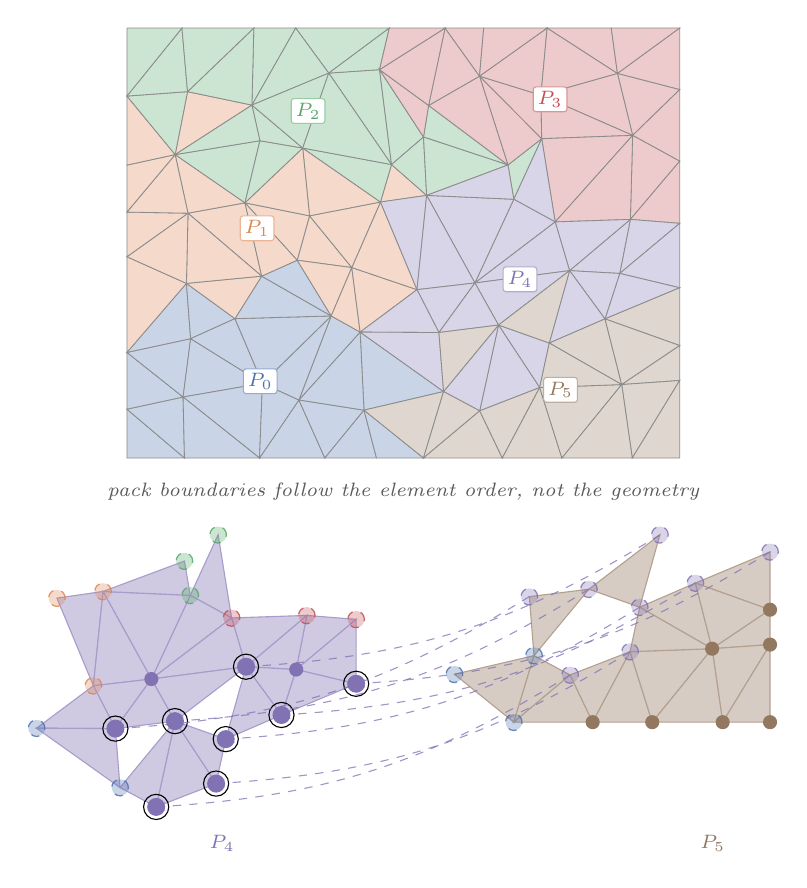
\begin{tikzpicture}[scale=0.78]
  \filldraw[fill=PackA!30,draw=black!45,line width=0.3pt,fill opacity=1.00] (0.000,0.000) -- (0.937,0.000) -- (0.000,0.795) -- cycle;
  \filldraw[fill=PackA!30,draw=black!45,line width=0.3pt,fill opacity=1.00] (0.937,0.000) -- (0.914,0.993) -- (0.000,0.795) -- cycle;
  \filldraw[fill=PackA!30,draw=black!45,line width=0.3pt,fill opacity=1.00] (0.000,0.795) -- (0.914,0.993) -- (0.000,1.719) -- cycle;
  \filldraw[fill=PackA!30,draw=black!45,line width=0.3pt,fill opacity=1.00] (0.914,0.993) -- (1.037,1.943) -- (0.000,1.719) -- cycle;
  \filldraw[fill=PackA!30,draw=black!45,line width=0.3pt,fill opacity=1.00] (0.000,1.719) -- (1.037,1.943) -- (0.969,2.843) -- cycle;
  \filldraw[fill=PackA!30,draw=black!45,line width=0.3pt,fill opacity=1.00] (1.037,1.943) -- (1.759,2.269) -- (0.969,2.843) -- cycle;
  \filldraw[fill=PackA!30,draw=black!45,line width=0.3pt,fill opacity=1.00] (0.914,0.993) -- (2.206,1.217) -- (1.037,1.943) -- cycle;
  \filldraw[fill=PackA!30,draw=black!45,line width=0.3pt,fill opacity=1.00] (2.206,1.217) -- (1.759,2.269) -- (1.037,1.943) -- cycle;
  \filldraw[fill=PackA!30,draw=black!45,line width=0.3pt,fill opacity=1.00] (2.159,0.000) -- (2.206,1.217) -- (0.914,0.993) -- cycle;
  \filldraw[fill=PackA!30,draw=black!45,line width=0.3pt,fill opacity=1.00] (0.937,0.000) -- (2.159,0.000) -- (0.914,0.993) -- cycle;
  \filldraw[fill=PackA!30,draw=black!45,line width=0.3pt,fill opacity=1.00] (2.159,0.000) -- (3.222,0.000) -- (2.800,0.945) -- cycle;
  \filldraw[fill=PackA!30,draw=black!45,line width=0.3pt,fill opacity=1.00] (2.159,0.000) -- (2.800,0.945) -- (2.206,1.217) -- cycle;
  \filldraw[fill=PackA!30,draw=black!45,line width=0.3pt,fill opacity=1.00] (3.222,0.000) -- (3.860,0.779) -- (2.800,0.945) -- cycle;
  \filldraw[fill=PackA!30,draw=black!45,line width=0.3pt,fill opacity=1.00] (3.222,0.000) -- (4.063,0.000) -- (3.860,0.779) -- cycle;
  \filldraw[fill=PackA!30,draw=black!45,line width=0.3pt,fill opacity=1.00] (4.063,0.000) -- (4.828,0.000) -- (3.860,0.779) -- cycle;
  \filldraw[fill=PackA!30,draw=black!45,line width=0.3pt,fill opacity=1.00] (3.860,0.779) -- (5.156,1.082) -- (3.797,2.050) -- cycle;
  \filldraw[fill=PackA!30,draw=black!45,line width=0.3pt,fill opacity=1.00] (2.800,0.945) -- (3.860,0.779) -- (3.797,2.050) -- cycle;
  \filldraw[fill=PackA!30,draw=black!45,line width=0.3pt,fill opacity=1.00] (2.800,0.945) -- (3.797,2.050) -- (3.326,2.313) -- cycle;
  \filldraw[fill=PackA!30,draw=black!45,line width=0.3pt,fill opacity=1.00] (2.206,1.217) -- (2.800,0.945) -- (3.326,2.313) -- cycle;
  \filldraw[fill=PackA!30,draw=black!45,line width=0.3pt,fill opacity=1.00] (2.206,1.217) -- (3.326,2.313) -- (1.759,2.269) -- cycle;
  \filldraw[fill=PackA!30,draw=black!45,line width=0.3pt,fill opacity=1.00] (1.759,2.269) -- (3.326,2.313) -- (2.194,2.961) -- cycle;
  \filldraw[fill=PackA!30,draw=black!45,line width=0.3pt,fill opacity=1.00] (3.326,2.313) -- (2.772,3.220) -- (2.194,2.961) -- cycle;
  \filldraw[fill=PackB!30,draw=black!45,line width=0.3pt,fill opacity=1.00] (2.772,3.220) -- (3.661,3.101) -- (2.973,3.943) -- cycle;
  \filldraw[fill=PackB!30,draw=black!45,line width=0.3pt,fill opacity=1.00] (3.326,2.313) -- (3.661,3.101) -- (2.772,3.220) -- cycle;
  \filldraw[fill=PackB!30,draw=black!45,line width=0.3pt,fill opacity=1.00] (3.326,2.313) -- (3.797,2.050) -- (3.661,3.101) -- cycle;
  \filldraw[fill=PackB!30,draw=black!45,line width=0.3pt,fill opacity=1.00] (3.797,2.050) -- (4.723,2.741) -- (3.661,3.101) -- cycle;
  \filldraw[fill=PackB!30,draw=black!45,line width=0.3pt,fill opacity=1.00] (3.661,3.101) -- (4.723,2.741) -- (4.128,4.168) -- cycle;
  \filldraw[fill=PackB!30,draw=black!45,line width=0.3pt,fill opacity=1.00] (3.661,3.101) -- (4.128,4.168) -- (2.973,3.943) -- cycle;
  \filldraw[fill=PackB!30,draw=black!45,line width=0.3pt,fill opacity=1.00] (4.128,4.168) -- (4.880,4.276) -- (4.308,4.778) -- cycle;
  \filldraw[fill=PackB!30,draw=black!45,line width=0.3pt,fill opacity=1.00] (2.973,3.943) -- (4.128,4.168) -- (2.862,5.047) -- cycle;
  \filldraw[fill=PackB!30,draw=black!45,line width=0.3pt,fill opacity=1.00] (2.772,3.220) -- (2.973,3.943) -- (1.922,4.155) -- cycle;
  \filldraw[fill=PackB!30,draw=black!45,line width=0.3pt,fill opacity=1.00] (1.922,4.155) -- (2.973,3.943) -- (2.862,5.047) -- cycle;
  \filldraw[fill=PackB!30,draw=black!45,line width=0.3pt,fill opacity=1.00] (2.194,2.961) -- (1.922,4.155) -- (0.994,3.986) -- cycle;
  \filldraw[fill=PackB!30,draw=black!45,line width=0.3pt,fill opacity=1.00] (2.194,2.961) -- (2.772,3.220) -- (1.922,4.155) -- cycle;
  \filldraw[fill=PackB!30,draw=black!45,line width=0.3pt,fill opacity=1.00] (1.759,2.269) -- (2.194,2.961) -- (0.969,2.843) -- cycle;
  \filldraw[fill=PackB!30,draw=black!45,line width=0.3pt,fill opacity=1.00] (0.969,2.843) -- (2.194,2.961) -- (0.994,3.986) -- cycle;
  \filldraw[fill=PackB!30,draw=black!45,line width=0.3pt,fill opacity=1.00] (0.000,1.719) -- (0.969,2.843) -- (0.000,3.277) -- cycle;
  \filldraw[fill=PackB!30,draw=black!45,line width=0.3pt,fill opacity=1.00] (0.000,3.277) -- (0.969,2.843) -- (0.994,3.986) -- cycle;
  \filldraw[fill=PackB!30,draw=black!45,line width=0.3pt,fill opacity=1.00] (0.000,3.277) -- (0.994,3.986) -- (0.000,4.004) -- cycle;
  \filldraw[fill=PackB!30,draw=black!45,line width=0.3pt,fill opacity=1.00] (0.994,3.986) -- (1.922,4.155) -- (0.785,4.940) -- cycle;
  \filldraw[fill=PackB!30,draw=black!45,line width=0.3pt,fill opacity=1.00] (0.000,4.004) -- (0.994,3.986) -- (0.785,4.940) -- cycle;
  \filldraw[fill=PackB!30,draw=black!45,line width=0.3pt,fill opacity=1.00] (0.000,4.004) -- (0.785,4.940) -- (0.000,4.769) -- cycle;
  \filldraw[fill=PackB!30,draw=black!45,line width=0.3pt,fill opacity=1.00] (0.000,4.769) -- (0.785,4.940) -- (0.000,5.893) -- cycle;
  \filldraw[fill=PackB!30,draw=black!45,line width=0.3pt,fill opacity=1.00] (0.785,4.940) -- (2.035,5.746) -- (0.987,5.965) -- cycle;
  \filldraw[fill=PackC!30,draw=black!45,line width=0.3pt,fill opacity=1.00] (1.922,4.155) -- (2.165,5.166) -- (0.785,4.940) -- cycle;
  \filldraw[fill=PackC!30,draw=black!45,line width=0.3pt,fill opacity=1.00] (1.922,4.155) -- (2.862,5.047) -- (2.165,5.166) -- cycle;
  \filldraw[fill=PackC!30,draw=black!45,line width=0.3pt,fill opacity=1.00] (2.165,5.166) -- (2.862,5.047) -- (2.035,5.746) -- cycle;
  \filldraw[fill=PackC!30,draw=black!45,line width=0.3pt,fill opacity=1.00] (0.785,4.940) -- (2.165,5.166) -- (2.035,5.746) -- cycle;
  \filldraw[fill=PackC!30,draw=black!45,line width=0.3pt,fill opacity=1.00] (2.035,5.746) -- (2.748,7.000) -- (2.066,7.000) -- cycle;
  \filldraw[fill=PackC!30,draw=black!45,line width=0.3pt,fill opacity=1.00] (0.987,5.965) -- (2.035,5.746) -- (2.066,7.000) -- cycle;
  \filldraw[fill=PackC!30,draw=black!45,line width=0.3pt,fill opacity=1.00] (0.785,4.940) -- (0.987,5.965) -- (0.000,5.893) -- cycle;
  \filldraw[fill=PackC!30,draw=black!45,line width=0.3pt,fill opacity=1.00] (0.000,5.893) -- (0.987,5.965) -- (0.896,7.000) -- cycle;
  \filldraw[fill=PackC!30,draw=black!45,line width=0.3pt,fill opacity=1.00] (0.000,5.893) -- (0.896,7.000) -- (0.000,7.000) -- cycle;
  \filldraw[fill=PackC!30,draw=black!45,line width=0.3pt,fill opacity=1.00] (0.987,5.965) -- (2.066,7.000) -- (0.896,7.000) -- cycle;
  \filldraw[fill=PackC!30,draw=black!45,line width=0.3pt,fill opacity=1.00] (3.286,6.267) -- (4.272,7.000) -- (2.748,7.000) -- cycle;
  \filldraw[fill=PackC!30,draw=black!45,line width=0.3pt,fill opacity=1.00] (4.308,4.778) -- (4.113,6.323) -- (3.286,6.267) -- cycle;
  \filldraw[fill=PackC!30,draw=black!45,line width=0.3pt,fill opacity=1.00] (3.286,6.267) -- (4.113,6.323) -- (4.272,7.000) -- cycle;
  \filldraw[fill=PackC!30,draw=black!45,line width=0.3pt,fill opacity=1.00] (2.035,5.746) -- (3.286,6.267) -- (2.748,7.000) -- cycle;
  \filldraw[fill=PackC!30,draw=black!45,line width=0.3pt,fill opacity=1.00] (2.862,5.047) -- (3.286,6.267) -- (2.035,5.746) -- cycle;
  \filldraw[fill=PackC!30,draw=black!45,line width=0.3pt,fill opacity=1.00] (4.128,4.168) -- (4.308,4.778) -- (2.862,5.047) -- cycle;
  \filldraw[fill=PackC!30,draw=black!45,line width=0.3pt,fill opacity=1.00] (2.862,5.047) -- (4.308,4.778) -- (3.286,6.267) -- cycle;
  \filldraw[fill=PackC!30,draw=black!45,line width=0.3pt,fill opacity=1.00] (4.308,4.778) -- (4.829,5.226) -- (4.113,6.323) -- cycle;
  \filldraw[fill=PackC!30,draw=black!45,line width=0.3pt,fill opacity=1.00] (4.880,4.276) -- (4.829,5.226) -- (4.308,4.778) -- cycle;
  \filldraw[fill=PackC!30,draw=black!45,line width=0.3pt,fill opacity=1.00] (4.829,5.226) -- (6.204,4.771) -- (4.912,5.740) -- cycle;
  \filldraw[fill=PackC!30,draw=black!45,line width=0.3pt,fill opacity=1.00] (4.880,4.276) -- (6.204,4.771) -- (4.829,5.226) -- cycle;
  \filldraw[fill=PackC!30,draw=black!45,line width=0.3pt,fill opacity=1.00] (6.299,4.213) -- (6.753,5.199) -- (6.204,4.771) -- cycle;
  \filldraw[fill=PackD!30,draw=black!45,line width=0.3pt,fill opacity=1.00] (6.204,4.771) -- (6.753,5.199) -- (5.741,6.217) -- cycle;
  \filldraw[fill=PackD!30,draw=black!45,line width=0.3pt,fill opacity=1.00] (6.204,4.771) -- (5.741,6.217) -- (4.912,5.740) -- cycle;
  \filldraw[fill=PackD!30,draw=black!45,line width=0.3pt,fill opacity=1.00] (6.753,5.199) -- (6.741,5.908) -- (5.741,6.217) -- cycle;
  \filldraw[fill=PackD!30,draw=black!45,line width=0.3pt,fill opacity=1.00] (5.741,6.217) -- (6.741,5.908) -- (6.841,7.000) -- cycle;
  \filldraw[fill=PackD!30,draw=black!45,line width=0.3pt,fill opacity=1.00] (4.912,5.740) -- (5.741,6.217) -- (5.180,7.000) -- cycle;
  \filldraw[fill=PackD!30,draw=black!45,line width=0.3pt,fill opacity=1.00] (4.829,5.226) -- (4.912,5.740) -- (4.113,6.323) -- cycle;
  \filldraw[fill=PackD!30,draw=black!45,line width=0.3pt,fill opacity=1.00] (4.113,6.323) -- (4.912,5.740) -- (5.180,7.000) -- cycle;
  \filldraw[fill=PackD!30,draw=black!45,line width=0.3pt,fill opacity=1.00] (4.113,6.323) -- (5.180,7.000) -- (4.272,7.000) -- cycle;
  \filldraw[fill=PackD!30,draw=black!45,line width=0.3pt,fill opacity=1.00] (5.741,6.217) -- (5.809,7.000) -- (5.180,7.000) -- cycle;
  \filldraw[fill=PackD!30,draw=black!45,line width=0.3pt,fill opacity=1.00] (5.741,6.217) -- (6.841,7.000) -- (5.809,7.000) -- cycle;
  \filldraw[fill=PackD!30,draw=black!45,line width=0.3pt,fill opacity=1.00] (7.987,6.260) -- (7.886,7.000) -- (6.841,7.000) -- cycle;
  \filldraw[fill=PackD!30,draw=black!45,line width=0.3pt,fill opacity=1.00] (7.987,6.260) -- (9.000,7.000) -- (7.886,7.000) -- cycle;
  \filldraw[fill=PackD!30,draw=black!45,line width=0.3pt,fill opacity=1.00] (7.987,6.260) -- (9.000,5.998) -- (9.000,7.000) -- cycle;
  \filldraw[fill=PackD!30,draw=black!45,line width=0.3pt,fill opacity=1.00] (8.234,5.253) -- (9.000,5.998) -- (7.987,6.260) -- cycle;
  \filldraw[fill=PackD!30,draw=black!45,line width=0.3pt,fill opacity=1.00] (6.741,5.908) -- (7.987,6.260) -- (6.841,7.000) -- cycle;
  \filldraw[fill=PackD!30,draw=black!45,line width=0.3pt,fill opacity=1.00] (8.234,5.253) -- (7.987,6.260) -- (6.741,5.908) -- cycle;
  \filldraw[fill=PackD!30,draw=black!45,line width=0.3pt,fill opacity=1.00] (6.753,5.199) -- (8.234,5.253) -- (6.741,5.908) -- cycle;
  \filldraw[fill=PackD!30,draw=black!45,line width=0.3pt,fill opacity=1.00] (6.973,3.844) -- (8.234,5.253) -- (6.753,5.199) -- cycle;
  \filldraw[fill=PackD!30,draw=black!45,line width=0.3pt,fill opacity=1.00] (8.234,5.253) -- (9.000,4.833) -- (9.000,5.998) -- cycle;
  \filldraw[fill=PackD!30,draw=black!45,line width=0.3pt,fill opacity=1.00] (8.197,3.885) -- (9.000,4.833) -- (8.234,5.253) -- cycle;
  \filldraw[fill=PackD!30,draw=black!45,line width=0.3pt,fill opacity=1.00] (8.197,3.885) -- (9.000,3.821) -- (9.000,4.833) -- cycle;
  \filldraw[fill=PackD!30,draw=black!45,line width=0.3pt,fill opacity=1.00] (6.973,3.844) -- (8.197,3.885) -- (8.234,5.253) -- cycle;
  \filldraw[fill=PackE!30,draw=black!45,line width=0.3pt,fill opacity=1.00] (8.024,3.005) -- (9.000,3.821) -- (8.197,3.885) -- cycle;
  \filldraw[fill=PackE!30,draw=black!45,line width=0.3pt,fill opacity=1.00] (8.024,3.005) -- (9.000,2.772) -- (9.000,3.821) -- cycle;
  \filldraw[fill=PackE!30,draw=black!45,line width=0.3pt,fill opacity=1.00] (7.784,2.265) -- (9.000,2.772) -- (8.024,3.005) -- cycle;
  \filldraw[fill=PackE!30,draw=black!45,line width=0.3pt,fill opacity=1.00] (7.207,3.051) -- (8.024,3.005) -- (8.197,3.885) -- cycle;
  \filldraw[fill=PackE!30,draw=black!45,line width=0.3pt,fill opacity=1.00] (7.784,2.265) -- (8.024,3.005) -- (7.207,3.051) -- cycle;
  \filldraw[fill=PackE!30,draw=black!45,line width=0.3pt,fill opacity=1.00] (6.877,1.872) -- (7.784,2.265) -- (7.207,3.051) -- cycle;
  \filldraw[fill=PackE!30,draw=black!45,line width=0.3pt,fill opacity=1.00] (7.207,3.051) -- (8.197,3.885) -- (6.973,3.844) -- cycle;
  \filldraw[fill=PackE!30,draw=black!45,line width=0.3pt,fill opacity=1.00] (6.299,4.213) -- (6.973,3.844) -- (6.753,5.199) -- cycle;
  \filldraw[fill=PackE!30,draw=black!45,line width=0.3pt,fill opacity=1.00] (5.666,2.850) -- (6.973,3.844) -- (6.299,4.213) -- cycle;
  \filldraw[fill=PackE!30,draw=black!45,line width=0.3pt,fill opacity=1.00] (5.666,2.850) -- (6.299,4.213) -- (4.880,4.276) -- cycle;
  \filldraw[fill=PackE!30,draw=black!45,line width=0.3pt,fill opacity=1.00] (4.880,4.276) -- (6.299,4.213) -- (6.204,4.771) -- cycle;
  \filldraw[fill=PackE!30,draw=black!45,line width=0.3pt,fill opacity=1.00] (4.723,2.741) -- (4.880,4.276) -- (4.128,4.168) -- cycle;
  \filldraw[fill=PackE!30,draw=black!45,line width=0.3pt,fill opacity=1.00] (4.723,2.741) -- (5.666,2.850) -- (4.880,4.276) -- cycle;
  \filldraw[fill=PackE!30,draw=black!45,line width=0.3pt,fill opacity=1.00] (5.080,2.043) -- (5.666,2.850) -- (4.723,2.741) -- cycle;
  \filldraw[fill=PackE!30,draw=black!45,line width=0.3pt,fill opacity=1.00] (5.666,2.850) -- (7.207,3.051) -- (6.973,3.844) -- cycle;
  \filldraw[fill=PackE!30,draw=black!45,line width=0.3pt,fill opacity=1.00] (6.050,2.165) -- (7.207,3.051) -- (5.666,2.850) -- cycle;
  \filldraw[fill=PackE!30,draw=black!45,line width=0.3pt,fill opacity=1.00] (6.720,1.147) -- (6.877,1.872) -- (6.050,2.165) -- cycle;
  \filldraw[fill=PackE!30,draw=black!45,line width=0.3pt,fill opacity=1.00] (5.744,0.768) -- (6.720,1.147) -- (6.050,2.165) -- cycle;
  \filldraw[fill=PackE!30,draw=black!45,line width=0.3pt,fill opacity=1.00] (5.156,1.082) -- (5.744,0.768) -- (6.050,2.165) -- cycle;
  \filldraw[fill=PackE!30,draw=black!45,line width=0.3pt,fill opacity=1.00] (5.080,2.043) -- (6.050,2.165) -- (5.666,2.850) -- cycle;
  \filldraw[fill=PackE!30,draw=black!45,line width=0.3pt,fill opacity=1.00] (3.797,2.050) -- (5.080,2.043) -- (4.723,2.741) -- cycle;
  \filldraw[fill=PackE!30,draw=black!45,line width=0.3pt,fill opacity=1.00] (5.156,1.082) -- (5.080,2.043) -- (3.797,2.050) -- cycle;
  \filldraw[fill=PackF!30,draw=black!45,line width=0.3pt,fill opacity=1.00] (5.156,1.082) -- (6.050,2.165) -- (5.080,2.043) -- cycle;
  \filldraw[fill=PackF!30,draw=black!45,line width=0.3pt,fill opacity=1.00] (4.828,0.000) -- (5.156,1.082) -- (3.860,0.779) -- cycle;
  \filldraw[fill=PackF!30,draw=black!45,line width=0.3pt,fill opacity=1.00] (4.828,0.000) -- (5.744,0.768) -- (5.156,1.082) -- cycle;
  \filldraw[fill=PackF!30,draw=black!45,line width=0.3pt,fill opacity=1.00] (4.828,0.000) -- (6.112,0.000) -- (5.744,0.768) -- cycle;
  \filldraw[fill=PackF!30,draw=black!45,line width=0.3pt,fill opacity=1.00] (6.112,0.000) -- (6.720,1.147) -- (5.744,0.768) -- cycle;
  \filldraw[fill=PackF!30,draw=black!45,line width=0.3pt,fill opacity=1.00] (6.112,0.000) -- (7.082,0.000) -- (6.720,1.147) -- cycle;
  \filldraw[fill=PackF!30,draw=black!45,line width=0.3pt,fill opacity=1.00] (7.082,0.000) -- (8.056,1.196) -- (6.720,1.147) -- cycle;
  \filldraw[fill=PackF!30,draw=black!45,line width=0.3pt,fill opacity=1.00] (6.050,2.165) -- (6.877,1.872) -- (7.207,3.051) -- cycle;
  \filldraw[fill=PackF!30,draw=black!45,line width=0.3pt,fill opacity=1.00] (8.056,1.196) -- (7.784,2.265) -- (6.877,1.872) -- cycle;
  \filldraw[fill=PackF!30,draw=black!45,line width=0.3pt,fill opacity=1.00] (6.720,1.147) -- (8.056,1.196) -- (6.877,1.872) -- cycle;
  \filldraw[fill=PackF!30,draw=black!45,line width=0.3pt,fill opacity=1.00] (7.784,2.265) -- (9.000,1.831) -- (9.000,2.772) -- cycle;
  \filldraw[fill=PackF!30,draw=black!45,line width=0.3pt,fill opacity=1.00] (8.056,1.196) -- (9.000,1.831) -- (7.784,2.265) -- cycle;
  \filldraw[fill=PackF!30,draw=black!45,line width=0.3pt,fill opacity=1.00] (8.056,1.196) -- (9.000,1.262) -- (9.000,1.831) -- cycle;
  \filldraw[fill=PackF!30,draw=black!45,line width=0.3pt,fill opacity=1.00] (8.228,0.000) -- (9.000,1.262) -- (8.056,1.196) -- cycle;
  \filldraw[fill=PackF!30,draw=black!45,line width=0.3pt,fill opacity=1.00] (7.082,0.000) -- (8.228,0.000) -- (8.056,1.196) -- cycle;
  \filldraw[fill=PackF!30,draw=black!45,line width=0.3pt,fill opacity=1.00] (8.228,0.000) -- (9.000,0.000) -- (9.000,1.262) -- cycle;
  \node[PackA,font=\bfseries\scriptsize,fill=white,inner sep=1.6pt,rounded corners=1pt,draw=PackA!60] at (2.17,1.25) {$P_0$};
  \node[PackB,font=\bfseries\scriptsize,fill=white,inner sep=1.6pt,rounded corners=1pt,draw=PackB!60] at (2.12,3.74) {$P_1$};
  \node[PackC,font=\bfseries\scriptsize,fill=white,inner sep=1.6pt,rounded corners=1pt,draw=PackC!60] at (2.95,5.65) {$P_2$};
  \node[PackD,font=\bfseries\scriptsize,fill=white,inner sep=1.6pt,rounded corners=1pt,draw=PackD!60] at (6.89,5.84) {$P_3$};
  \node[PackE,font=\bfseries\scriptsize,fill=white,inner sep=1.6pt,rounded corners=1pt,draw=PackE!60] at (6.40,2.91) {$P_4$};
  \node[PackF,font=\bfseries\scriptsize,fill=white,inner sep=1.6pt,rounded corners=1pt,draw=PackF!60] at (7.06,1.11) {$P_5$};
  \node[anchor=north,font=\scriptsize\itshape,black!65] at (4.50,-0.25) {pack boundaries follow the element order, not the geometry};
  \filldraw[fill=PackE!38,draw=PackE!70,line width=0.4pt,fill opacity=1.00] (2.756,-3.444) -- (3.732,-2.627) -- (2.929,-2.563) -- cycle;
  \filldraw[fill=PackE!38,draw=PackE!70,line width=0.4pt,fill opacity=1.00] (2.756,-3.444) -- (3.732,-3.676) -- (3.732,-2.627) -- cycle;
  \filldraw[fill=PackE!38,draw=PackE!70,line width=0.4pt,fill opacity=1.00] (2.516,-4.184) -- (3.732,-3.676) -- (2.756,-3.444) -- cycle;
  \filldraw[fill=PackE!38,draw=PackE!70,line width=0.4pt,fill opacity=1.00] (1.939,-3.398) -- (2.756,-3.444) -- (2.929,-2.563) -- cycle;
  \filldraw[fill=PackE!38,draw=PackE!70,line width=0.4pt,fill opacity=1.00] (2.516,-4.184) -- (2.756,-3.444) -- (1.939,-3.398) -- cycle;
  \filldraw[fill=PackE!38,draw=PackE!70,line width=0.4pt,fill opacity=1.00] (1.609,-4.577) -- (2.516,-4.184) -- (1.939,-3.398) -- cycle;
  \filldraw[fill=PackE!38,draw=PackE!70,line width=0.4pt,fill opacity=1.00] (1.939,-3.398) -- (2.929,-2.563) -- (1.704,-2.604) -- cycle;
  \filldraw[fill=PackE!38,draw=PackE!70,line width=0.4pt,fill opacity=1.00] (1.031,-2.236) -- (1.704,-2.604) -- (1.485,-1.250) -- cycle;
  \filldraw[fill=PackE!38,draw=PackE!70,line width=0.4pt,fill opacity=1.00] (0.398,-3.599) -- (1.704,-2.604) -- (1.031,-2.236) -- cycle;
  \filldraw[fill=PackE!38,draw=PackE!70,line width=0.4pt,fill opacity=1.00] (0.398,-3.599) -- (1.031,-2.236) -- (-0.389,-2.173) -- cycle;
  \filldraw[fill=PackE!38,draw=PackE!70,line width=0.4pt,fill opacity=1.00] (-0.389,-2.173) -- (1.031,-2.236) -- (0.936,-1.678) -- cycle;
  \filldraw[fill=PackE!38,draw=PackE!70,line width=0.4pt,fill opacity=1.00] (-0.546,-3.708) -- (-0.389,-2.173) -- (-1.140,-2.281) -- cycle;
  \filldraw[fill=PackE!38,draw=PackE!70,line width=0.4pt,fill opacity=1.00] (-0.546,-3.708) -- (0.398,-3.599) -- (-0.389,-2.173) -- cycle;
  \filldraw[fill=PackE!38,draw=PackE!70,line width=0.4pt,fill opacity=1.00] (-0.188,-4.406) -- (0.398,-3.599) -- (-0.546,-3.708) -- cycle;
  \filldraw[fill=PackE!38,draw=PackE!70,line width=0.4pt,fill opacity=1.00] (0.398,-3.599) -- (1.939,-3.398) -- (1.704,-2.604) -- cycle;
  \filldraw[fill=PackE!38,draw=PackE!70,line width=0.4pt,fill opacity=1.00] (0.782,-4.284) -- (1.939,-3.398) -- (0.398,-3.599) -- cycle;
  \filldraw[fill=PackE!38,draw=PackE!70,line width=0.4pt,fill opacity=1.00] (1.452,-5.301) -- (1.609,-4.577) -- (0.782,-4.284) -- cycle;
  \filldraw[fill=PackE!38,draw=PackE!70,line width=0.4pt,fill opacity=1.00] (0.476,-5.681) -- (1.452,-5.301) -- (0.782,-4.284) -- cycle;
  \filldraw[fill=PackE!38,draw=PackE!70,line width=0.4pt,fill opacity=1.00] (-0.112,-5.366) -- (0.476,-5.681) -- (0.782,-4.284) -- cycle;
  \filldraw[fill=PackE!38,draw=PackE!70,line width=0.4pt,fill opacity=1.00] (-0.188,-4.406) -- (0.782,-4.284) -- (0.398,-3.599) -- cycle;
  \filldraw[fill=PackE!38,draw=PackE!70,line width=0.4pt,fill opacity=1.00] (-1.471,-4.399) -- (-0.188,-4.406) -- (-0.546,-3.708) -- cycle;
  \filldraw[fill=PackE!38,draw=PackE!70,line width=0.4pt,fill opacity=1.00] (-0.112,-5.366) -- (-0.188,-4.406) -- (-1.471,-4.399) -- cycle;
  \fill[PackE] (0.398,-3.599) circle (0.115);
  \fill[PackE] (2.756,-3.444) circle (0.115);
  \draw[PackE,fill=PackE,line width=0.5pt] (0.476,-5.681) circle (0.135);
  \draw[black,line width=0.4pt] (0.476,-5.681) circle (0.205);
  \draw[PackE,fill=PackE,line width=0.5pt] (1.452,-5.301) circle (0.135);
  \draw[black,line width=0.4pt] (1.452,-5.301) circle (0.205);
  \draw[PackE,fill=PackE,line width=0.5pt] (-0.188,-4.406) circle (0.135);
  \draw[black,line width=0.4pt] (-0.188,-4.406) circle (0.205);
  \draw[PackE,fill=PackE,line width=0.5pt] (0.782,-4.284) circle (0.135);
  \draw[black,line width=0.4pt] (0.782,-4.284) circle (0.205);
  \draw[PackE,fill=PackE,line width=0.5pt] (1.609,-4.577) circle (0.135);
  \draw[black,line width=0.4pt] (1.609,-4.577) circle (0.205);
  \draw[PackE,fill=PackE,line width=0.5pt] (2.516,-4.184) circle (0.135);
  \draw[black,line width=0.4pt] (2.516,-4.184) circle (0.205);
  \draw[PackE,fill=PackE,line width=0.5pt] (1.939,-3.398) circle (0.135);
  \draw[black,line width=0.4pt] (1.939,-3.398) circle (0.205);
  \draw[PackE,fill=PackE,line width=0.5pt] (3.732,-3.676) circle (0.135);
  \draw[black,line width=0.4pt] (3.732,-3.676) circle (0.205);
  \filldraw[fill=PackC,draw=PackC,fill opacity=0.30,draw opacity=0.85,dashed,line width=0.45pt] (1.031,-2.236) circle (0.135);
  \filldraw[fill=PackB,draw=PackB,fill opacity=0.30,draw opacity=0.85,dashed,line width=0.45pt] (-0.389,-2.173) circle (0.135);
  \filldraw[fill=PackB,draw=PackB,fill opacity=0.30,draw opacity=0.85,dashed,line width=0.45pt] (-0.546,-3.708) circle (0.135);
  \filldraw[fill=PackA,draw=PackA,fill opacity=0.30,draw opacity=0.85,dashed,line width=0.45pt] (-0.112,-5.366) circle (0.135);
  \filldraw[fill=PackA,draw=PackA,fill opacity=0.30,draw opacity=0.85,dashed,line width=0.45pt] (-1.471,-4.399) circle (0.135);
  \filldraw[fill=PackD,draw=PackD,fill opacity=0.30,draw opacity=0.85,dashed,line width=0.45pt] (3.732,-2.627) circle (0.135);
  \filldraw[fill=PackD,draw=PackD,fill opacity=0.30,draw opacity=0.85,dashed,line width=0.45pt] (2.929,-2.563) circle (0.135);
  \filldraw[fill=PackD,draw=PackD,fill opacity=0.30,draw opacity=0.85,dashed,line width=0.45pt] (1.704,-2.604) circle (0.135);
  \filldraw[fill=PackC,draw=PackC,fill opacity=0.30,draw opacity=0.85,dashed,line width=0.45pt] (1.485,-1.250) circle (0.135);
  \filldraw[fill=PackC,draw=PackC,fill opacity=0.30,draw opacity=0.85,dashed,line width=0.45pt] (0.936,-1.678) circle (0.135);
  \filldraw[fill=PackB,draw=PackB,fill opacity=0.30,draw opacity=0.85,dashed,line width=0.45pt] (-1.140,-2.281) circle (0.135);
  \node[PackE,font=\bfseries\scriptsize,anchor=north] at (1.55,-5.98) {$P_4$};
  \filldraw[fill=PackF!38,draw=PackF!70,line width=0.4pt,fill opacity=1.00] (6.628,-3.218) -- (7.522,-2.136) -- (6.552,-2.257) -- cycle;
  \filldraw[fill=PackF!38,draw=PackF!70,line width=0.4pt,fill opacity=1.00] (6.299,-4.301) -- (6.628,-3.218) -- (5.332,-3.521) -- cycle;
  \filldraw[fill=PackF!38,draw=PackF!70,line width=0.4pt,fill opacity=1.00] (6.299,-4.301) -- (7.216,-3.532) -- (6.628,-3.218) -- cycle;
  \filldraw[fill=PackF!38,draw=PackF!70,line width=0.4pt,fill opacity=1.00] (6.299,-4.301) -- (7.583,-4.301) -- (7.216,-3.532) -- cycle;
  \filldraw[fill=PackF!38,draw=PackF!70,line width=0.4pt,fill opacity=1.00] (7.583,-4.301) -- (8.192,-3.153) -- (7.216,-3.532) -- cycle;
  \filldraw[fill=PackF!38,draw=PackF!70,line width=0.4pt,fill opacity=1.00] (7.583,-4.301) -- (8.553,-4.301) -- (8.192,-3.153) -- cycle;
  \filldraw[fill=PackF!38,draw=PackF!70,line width=0.4pt,fill opacity=1.00] (8.553,-4.301) -- (9.528,-3.105) -- (8.192,-3.153) -- cycle;
  \filldraw[fill=PackF!38,draw=PackF!70,line width=0.4pt,fill opacity=1.00] (7.522,-2.136) -- (8.349,-2.429) -- (8.678,-1.250) -- cycle;
  \filldraw[fill=PackF!38,draw=PackF!70,line width=0.4pt,fill opacity=1.00] (9.528,-3.105) -- (9.256,-2.036) -- (8.349,-2.429) -- cycle;
  \filldraw[fill=PackF!38,draw=PackF!70,line width=0.4pt,fill opacity=1.00] (8.192,-3.153) -- (9.528,-3.105) -- (8.349,-2.429) -- cycle;
  \filldraw[fill=PackF!38,draw=PackF!70,line width=0.4pt,fill opacity=1.00] (9.256,-2.036) -- (10.471,-2.470) -- (10.471,-1.528) -- cycle;
  \filldraw[fill=PackF!38,draw=PackF!70,line width=0.4pt,fill opacity=1.00] (9.528,-3.105) -- (10.471,-2.470) -- (9.256,-2.036) -- cycle;
  \filldraw[fill=PackF!38,draw=PackF!70,line width=0.4pt,fill opacity=1.00] (9.528,-3.105) -- (10.471,-3.038) -- (10.471,-2.470) -- cycle;
  \filldraw[fill=PackF!38,draw=PackF!70,line width=0.4pt,fill opacity=1.00] (9.700,-4.301) -- (10.471,-3.038) -- (9.528,-3.105) -- cycle;
  \filldraw[fill=PackF!38,draw=PackF!70,line width=0.4pt,fill opacity=1.00] (8.553,-4.301) -- (9.700,-4.301) -- (9.528,-3.105) -- cycle;
  \filldraw[fill=PackF!38,draw=PackF!70,line width=0.4pt,fill opacity=1.00] (9.700,-4.301) -- (10.471,-4.301) -- (10.471,-3.038) -- cycle;
  \fill[PackF] (7.583,-4.301) circle (0.115);
  \fill[PackF] (8.553,-4.301) circle (0.115);
  \fill[PackF] (9.700,-4.301) circle (0.115);
  \fill[PackF] (10.471,-4.301) circle (0.115);
  \fill[PackF] (9.528,-3.105) circle (0.115);
  \fill[PackF] (10.471,-3.038) circle (0.115);
  \fill[PackF] (10.471,-2.470) circle (0.115);
  \filldraw[fill=PackA,draw=PackA,fill opacity=0.30,draw opacity=0.85,dashed,line width=0.45pt] (6.628,-3.218) circle (0.135);
  \filldraw[fill=PackA,draw=PackA,fill opacity=0.30,draw opacity=0.85,dashed,line width=0.45pt] (6.299,-4.301) circle (0.135);
  \filldraw[fill=PackE,draw=PackE,fill opacity=0.30,draw opacity=0.85,dashed,line width=0.45pt] (7.522,-2.136) circle (0.135);
  \filldraw[fill=PackE,draw=PackE,fill opacity=0.30,draw opacity=0.85,dashed,line width=0.45pt] (8.192,-3.153) circle (0.135);
  \filldraw[fill=PackE,draw=PackE,fill opacity=0.30,draw opacity=0.85,dashed,line width=0.45pt] (9.256,-2.036) circle (0.135);
  \filldraw[fill=PackE,draw=PackE,fill opacity=0.30,draw opacity=0.85,dashed,line width=0.45pt] (7.216,-3.532) circle (0.135);
  \filldraw[fill=PackE,draw=PackE,fill opacity=0.30,draw opacity=0.85,dashed,line width=0.45pt] (8.349,-2.429) circle (0.135);
  \filldraw[fill=PackE,draw=PackE,fill opacity=0.30,draw opacity=0.85,dashed,line width=0.45pt] (6.552,-2.257) circle (0.135);
  \filldraw[fill=PackA,draw=PackA,fill opacity=0.30,draw opacity=0.85,dashed,line width=0.45pt] (5.332,-3.521) circle (0.135);
  \filldraw[fill=PackE,draw=PackE,fill opacity=0.30,draw opacity=0.85,dashed,line width=0.45pt] (8.678,-1.250) circle (0.135);
  \filldraw[fill=PackE,draw=PackE,fill opacity=0.30,draw opacity=0.85,dashed,line width=0.45pt] (10.471,-1.528) circle (0.135);
  \node[PackF,font=\bfseries\scriptsize,anchor=north] at (9.54,-5.98) {$P_5$};
  \draw[PackE,dashed,line width=0.4pt,draw opacity=0.75,->,>=stealth,bend left=14] (7.522,-2.136) to[bend left=14] (0.782,-4.284);
  \draw[PackE,dashed,line width=0.4pt,draw opacity=0.75,->,>=stealth,bend left=14] (8.192,-3.153) to[bend left=14] (1.452,-5.301);
  \draw[PackE,dashed,line width=0.4pt,draw opacity=0.75,->,>=stealth,bend left=14] (9.256,-2.036) to[bend left=14] (2.516,-4.184);
  \draw[PackE,dashed,line width=0.4pt,draw opacity=0.75,->,>=stealth,bend left=14] (7.216,-3.532) to[bend left=14] (0.476,-5.681);
  \draw[PackE,dashed,line width=0.4pt,draw opacity=0.75,->,>=stealth,bend left=14] (8.349,-2.429) to[bend left=14] (1.609,-4.577);
  \draw[PackE,dashed,line width=0.4pt,draw opacity=0.75,->,>=stealth,bend left=14] (6.552,-2.257) to[bend left=14] (-0.188,-4.406);
  \draw[PackE,dashed,line width=0.4pt,draw opacity=0.75,->,>=stealth,bend left=14] (8.678,-1.250) to[bend left=14] (1.939,-3.398);
  \draw[PackE,dashed,line width=0.4pt,draw opacity=0.75,->,>=stealth,bend left=14] (10.471,-1.528) to[bend left=14] (3.732,-3.676);
\end{tikzpicture}
}
  \caption{A mesh of $\figPackNx\times\figPackNy$ elements in $\figPackNPacks$ packs of
    $\figPackElemsPerPack$, after space-filling reordering. Element tint gives the
    pack. A filled node is owned by the pack of its colour and touched by no other pack; a
    ringed node is owned by the pack of its colour and \emph{also touched} by at least one
    other, which is what the ghost machinery of \S\ref{sec:format:ghost} exists to close. The
    figure is generated by reimplementing the format's documented ownership rules, not drawn,
    so it cannot disagree with them; two dimensions are used because a readable picture of a
    three-dimensional pack decomposition does not exist.}
  \label{fig:decomposition}
\end{figure}

\subsection{Node identity: one owner, three zones}
\label{sec:format:zones}

Each node has exactly one owning pack, and pack $p$ owns a contiguous, monotonically increasing
range of global indices. The owned ranges therefore \emph{partition} $[0, n_{\mathrm{nodes}})$.
Writing $n_c(p)$ for the size of that range, a pack-local index $\ell$ resolves to a global one
as
\[
  g(p,\ell) =
  \begin{cases}
    \texttt{owned\_nodes\_ptr}[p] + \ell, & \ell < n_c(p),\\[2pt]
    \texttt{ghost\_idx}\big[\texttt{ghost\_ptr}[p] + \ell - n_c(p)\big], & \ell \ge n_c(p).
  \end{cases}
\]
Because the owned ranges are contiguous and monotone in $p$, the owner of a global index is
recoverable by binary search, which is what lets a conflict graph over packs be built without
storing one.

The pack-local index is a \textbf{16-bit unsigned integer}. That is the single most consequential
choice in the format and it cuts both ways: it halves the index traffic of the element sweep
against the \SI{32}{\bit} global index a flat sweep must use (\S\ref{sec:cost}), and it caps a
pack at $2^{16}$ distinct nodes, which is what bounds the pack size and, as
\S\ref{sec:res:packsize} shows, is also what the packer wrongly uses to choose one.

Within the owned range the indices are ordered \emph{non-shared first, then shared}. With
$n_s(p)$ the number of a pack's owned nodes that some other pack also touches, the local index
space splits into three zones (Figure~\ref{fig:idspace}):
\begin{center}
\begin{tabular}{ll}
\toprule
range of $\ell$ & property \\
\midrule
$0 \le \ell < n_c - n_s$ & owned, touched by no other pack \\
$n_c - n_s \le \ell < n_c$ & owned, also touched elsewhere \\
$n_c \le \ell < n_{\mathrm{pack}}$ & ghost: touched, not owned \\
\bottomrule
\end{tabular}
\end{center}

This split is the least obvious property of the format. On a CPU, where one thread owns a pack,
the whole flush of the owned range is already contention-free and the distinction is not needed;
it becomes load-bearing wherever a pack is processed by more than one thread, since the first
zone can then be written without synchronisation and only the shared tail cannot.

\begin{figure}[t]
  \centering
  \resizebox{\columnwidth}{!}{% Generated by wip/paper/python/packed_format_figures.py -- do not edit.
% Regenerate with: make figures

\definecolor{PackA}{HTML}{4C72B0}
\definecolor{PackB}{HTML}{DD8452}
\definecolor{PackC}{HTML}{55A868}
\definecolor{PackD}{HTML}{C44E52}
\definecolor{PackE}{HTML}{8172B3}
\definecolor{PackF}{HTML}{937860}

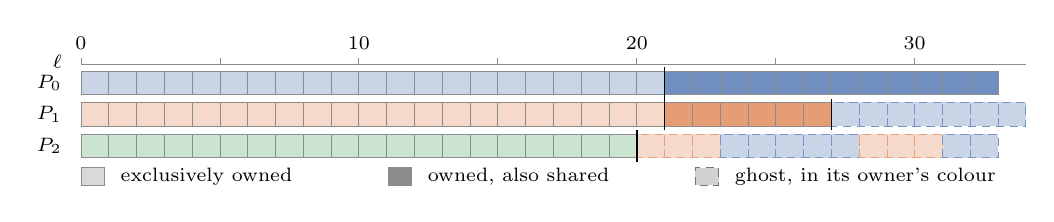
\begin{tikzpicture}[scale=1.00]
  \fill[PackA!30] (0.000,0.800) rectangle (0.353,1.100);
  \draw[black!45,line width=0.3pt] (0.000,0.800) rectangle (0.353,1.100);
  \fill[PackA!30] (0.353,0.800) rectangle (0.706,1.100);
  \draw[black!45,line width=0.3pt] (0.353,0.800) rectangle (0.706,1.100);
  \fill[PackA!30] (0.706,0.800) rectangle (1.059,1.100);
  \draw[black!45,line width=0.3pt] (0.706,0.800) rectangle (1.059,1.100);
  \fill[PackA!30] (1.059,0.800) rectangle (1.412,1.100);
  \draw[black!45,line width=0.3pt] (1.059,0.800) rectangle (1.412,1.100);
  \fill[PackA!30] (1.412,0.800) rectangle (1.765,1.100);
  \draw[black!45,line width=0.3pt] (1.412,0.800) rectangle (1.765,1.100);
  \fill[PackA!30] (1.765,0.800) rectangle (2.118,1.100);
  \draw[black!45,line width=0.3pt] (1.765,0.800) rectangle (2.118,1.100);
  \fill[PackA!30] (2.118,0.800) rectangle (2.471,1.100);
  \draw[black!45,line width=0.3pt] (2.118,0.800) rectangle (2.471,1.100);
  \fill[PackA!30] (2.471,0.800) rectangle (2.824,1.100);
  \draw[black!45,line width=0.3pt] (2.471,0.800) rectangle (2.824,1.100);
  \fill[PackA!30] (2.824,0.800) rectangle (3.176,1.100);
  \draw[black!45,line width=0.3pt] (2.824,0.800) rectangle (3.176,1.100);
  \fill[PackA!30] (3.176,0.800) rectangle (3.529,1.100);
  \draw[black!45,line width=0.3pt] (3.176,0.800) rectangle (3.529,1.100);
  \fill[PackA!30] (3.529,0.800) rectangle (3.882,1.100);
  \draw[black!45,line width=0.3pt] (3.529,0.800) rectangle (3.882,1.100);
  \fill[PackA!30] (3.882,0.800) rectangle (4.235,1.100);
  \draw[black!45,line width=0.3pt] (3.882,0.800) rectangle (4.235,1.100);
  \fill[PackA!30] (4.235,0.800) rectangle (4.588,1.100);
  \draw[black!45,line width=0.3pt] (4.235,0.800) rectangle (4.588,1.100);
  \fill[PackA!30] (4.588,0.800) rectangle (4.941,1.100);
  \draw[black!45,line width=0.3pt] (4.588,0.800) rectangle (4.941,1.100);
  \fill[PackA!30] (4.941,0.800) rectangle (5.294,1.100);
  \draw[black!45,line width=0.3pt] (4.941,0.800) rectangle (5.294,1.100);
  \fill[PackA!30] (5.294,0.800) rectangle (5.647,1.100);
  \draw[black!45,line width=0.3pt] (5.294,0.800) rectangle (5.647,1.100);
  \fill[PackA!30] (5.647,0.800) rectangle (6.000,1.100);
  \draw[black!45,line width=0.3pt] (5.647,0.800) rectangle (6.000,1.100);
  \fill[PackA!30] (6.000,0.800) rectangle (6.353,1.100);
  \draw[black!45,line width=0.3pt] (6.000,0.800) rectangle (6.353,1.100);
  \fill[PackA!30] (6.353,0.800) rectangle (6.706,1.100);
  \draw[black!45,line width=0.3pt] (6.353,0.800) rectangle (6.706,1.100);
  \fill[PackA!30] (6.706,0.800) rectangle (7.059,1.100);
  \draw[black!45,line width=0.3pt] (6.706,0.800) rectangle (7.059,1.100);
  \fill[PackA!30] (7.059,0.800) rectangle (7.412,1.100);
  \draw[black!45,line width=0.3pt] (7.059,0.800) rectangle (7.412,1.100);
  \fill[PackA!80] (7.412,0.800) rectangle (7.765,1.100);
  \draw[black!45,line width=0.3pt] (7.412,0.800) rectangle (7.765,1.100);
  \fill[PackA!80] (7.765,0.800) rectangle (8.118,1.100);
  \draw[black!45,line width=0.3pt] (7.765,0.800) rectangle (8.118,1.100);
  \fill[PackA!80] (8.118,0.800) rectangle (8.471,1.100);
  \draw[black!45,line width=0.3pt] (8.118,0.800) rectangle (8.471,1.100);
  \fill[PackA!80] (8.471,0.800) rectangle (8.824,1.100);
  \draw[black!45,line width=0.3pt] (8.471,0.800) rectangle (8.824,1.100);
  \fill[PackA!80] (8.824,0.800) rectangle (9.176,1.100);
  \draw[black!45,line width=0.3pt] (8.824,0.800) rectangle (9.176,1.100);
  \fill[PackA!80] (9.176,0.800) rectangle (9.529,1.100);
  \draw[black!45,line width=0.3pt] (9.176,0.800) rectangle (9.529,1.100);
  \fill[PackA!80] (9.529,0.800) rectangle (9.882,1.100);
  \draw[black!45,line width=0.3pt] (9.529,0.800) rectangle (9.882,1.100);
  \fill[PackA!80] (9.882,0.800) rectangle (10.235,1.100);
  \draw[black!45,line width=0.3pt] (9.882,0.800) rectangle (10.235,1.100);
  \fill[PackA!80] (10.235,0.800) rectangle (10.588,1.100);
  \draw[black!45,line width=0.3pt] (10.235,0.800) rectangle (10.588,1.100);
  \fill[PackA!80] (10.588,0.800) rectangle (10.941,1.100);
  \draw[black!45,line width=0.3pt] (10.588,0.800) rectangle (10.941,1.100);
  \fill[PackA!80] (10.941,0.800) rectangle (11.294,1.100);
  \draw[black!45,line width=0.3pt] (10.941,0.800) rectangle (11.294,1.100);
  \fill[PackA!80] (11.294,0.800) rectangle (11.647,1.100);
  \draw[black!45,line width=0.3pt] (11.294,0.800) rectangle (11.647,1.100);
  \draw[black,line width=0.55pt] (7.412,0.750) -- (7.412,1.150);
  \node[font=\scriptsize,anchor=east] at (-0.12,0.950) {$P_{0}$};
  \fill[PackB!30] (0.000,0.400) rectangle (0.353,0.700);
  \draw[black!45,line width=0.3pt] (0.000,0.400) rectangle (0.353,0.700);
  \fill[PackB!30] (0.353,0.400) rectangle (0.706,0.700);
  \draw[black!45,line width=0.3pt] (0.353,0.400) rectangle (0.706,0.700);
  \fill[PackB!30] (0.706,0.400) rectangle (1.059,0.700);
  \draw[black!45,line width=0.3pt] (0.706,0.400) rectangle (1.059,0.700);
  \fill[PackB!30] (1.059,0.400) rectangle (1.412,0.700);
  \draw[black!45,line width=0.3pt] (1.059,0.400) rectangle (1.412,0.700);
  \fill[PackB!30] (1.412,0.400) rectangle (1.765,0.700);
  \draw[black!45,line width=0.3pt] (1.412,0.400) rectangle (1.765,0.700);
  \fill[PackB!30] (1.765,0.400) rectangle (2.118,0.700);
  \draw[black!45,line width=0.3pt] (1.765,0.400) rectangle (2.118,0.700);
  \fill[PackB!30] (2.118,0.400) rectangle (2.471,0.700);
  \draw[black!45,line width=0.3pt] (2.118,0.400) rectangle (2.471,0.700);
  \fill[PackB!30] (2.471,0.400) rectangle (2.824,0.700);
  \draw[black!45,line width=0.3pt] (2.471,0.400) rectangle (2.824,0.700);
  \fill[PackB!30] (2.824,0.400) rectangle (3.176,0.700);
  \draw[black!45,line width=0.3pt] (2.824,0.400) rectangle (3.176,0.700);
  \fill[PackB!30] (3.176,0.400) rectangle (3.529,0.700);
  \draw[black!45,line width=0.3pt] (3.176,0.400) rectangle (3.529,0.700);
  \fill[PackB!30] (3.529,0.400) rectangle (3.882,0.700);
  \draw[black!45,line width=0.3pt] (3.529,0.400) rectangle (3.882,0.700);
  \fill[PackB!30] (3.882,0.400) rectangle (4.235,0.700);
  \draw[black!45,line width=0.3pt] (3.882,0.400) rectangle (4.235,0.700);
  \fill[PackB!30] (4.235,0.400) rectangle (4.588,0.700);
  \draw[black!45,line width=0.3pt] (4.235,0.400) rectangle (4.588,0.700);
  \fill[PackB!30] (4.588,0.400) rectangle (4.941,0.700);
  \draw[black!45,line width=0.3pt] (4.588,0.400) rectangle (4.941,0.700);
  \fill[PackB!30] (4.941,0.400) rectangle (5.294,0.700);
  \draw[black!45,line width=0.3pt] (4.941,0.400) rectangle (5.294,0.700);
  \fill[PackB!30] (5.294,0.400) rectangle (5.647,0.700);
  \draw[black!45,line width=0.3pt] (5.294,0.400) rectangle (5.647,0.700);
  \fill[PackB!30] (5.647,0.400) rectangle (6.000,0.700);
  \draw[black!45,line width=0.3pt] (5.647,0.400) rectangle (6.000,0.700);
  \fill[PackB!30] (6.000,0.400) rectangle (6.353,0.700);
  \draw[black!45,line width=0.3pt] (6.000,0.400) rectangle (6.353,0.700);
  \fill[PackB!30] (6.353,0.400) rectangle (6.706,0.700);
  \draw[black!45,line width=0.3pt] (6.353,0.400) rectangle (6.706,0.700);
  \fill[PackB!30] (6.706,0.400) rectangle (7.059,0.700);
  \draw[black!45,line width=0.3pt] (6.706,0.400) rectangle (7.059,0.700);
  \fill[PackB!30] (7.059,0.400) rectangle (7.412,0.700);
  \draw[black!45,line width=0.3pt] (7.059,0.400) rectangle (7.412,0.700);
  \fill[PackB!80] (7.412,0.400) rectangle (7.765,0.700);
  \draw[black!45,line width=0.3pt] (7.412,0.400) rectangle (7.765,0.700);
  \fill[PackB!80] (7.765,0.400) rectangle (8.118,0.700);
  \draw[black!45,line width=0.3pt] (7.765,0.400) rectangle (8.118,0.700);
  \fill[PackB!80] (8.118,0.400) rectangle (8.471,0.700);
  \draw[black!45,line width=0.3pt] (8.118,0.400) rectangle (8.471,0.700);
  \fill[PackB!80] (8.471,0.400) rectangle (8.824,0.700);
  \draw[black!45,line width=0.3pt] (8.471,0.400) rectangle (8.824,0.700);
  \fill[PackB!80] (8.824,0.400) rectangle (9.176,0.700);
  \draw[black!45,line width=0.3pt] (8.824,0.400) rectangle (9.176,0.700);
  \fill[PackB!80] (9.176,0.400) rectangle (9.529,0.700);
  \draw[black!45,line width=0.3pt] (9.176,0.400) rectangle (9.529,0.700);
  \fill[PackA!75,fill opacity=0.40] (9.529,0.400) rectangle (9.882,0.700);
  \draw[PackA!75,densely dashed,line width=0.3pt] (9.529,0.400) rectangle (9.882,0.700);
  \fill[PackA!75,fill opacity=0.40] (9.882,0.400) rectangle (10.235,0.700);
  \draw[PackA!75,densely dashed,line width=0.3pt] (9.882,0.400) rectangle (10.235,0.700);
  \fill[PackA!75,fill opacity=0.40] (10.235,0.400) rectangle (10.588,0.700);
  \draw[PackA!75,densely dashed,line width=0.3pt] (10.235,0.400) rectangle (10.588,0.700);
  \fill[PackA!75,fill opacity=0.40] (10.588,0.400) rectangle (10.941,0.700);
  \draw[PackA!75,densely dashed,line width=0.3pt] (10.588,0.400) rectangle (10.941,0.700);
  \fill[PackA!75,fill opacity=0.40] (10.941,0.400) rectangle (11.294,0.700);
  \draw[PackA!75,densely dashed,line width=0.3pt] (10.941,0.400) rectangle (11.294,0.700);
  \fill[PackA!75,fill opacity=0.40] (11.294,0.400) rectangle (11.647,0.700);
  \draw[PackA!75,densely dashed,line width=0.3pt] (11.294,0.400) rectangle (11.647,0.700);
  \fill[PackA!75,fill opacity=0.40] (11.647,0.400) rectangle (12.000,0.700);
  \draw[PackA!75,densely dashed,line width=0.3pt] (11.647,0.400) rectangle (12.000,0.700);
  \draw[black,line width=0.55pt] (7.412,0.350) -- (7.412,0.750);
  \draw[black,line width=0.55pt] (9.529,0.350) -- (9.529,0.750);
  \node[font=\scriptsize,anchor=east] at (-0.12,0.550) {$P_{1}$};
  \fill[PackC!30] (0.000,0.000) rectangle (0.353,0.300);
  \draw[black!45,line width=0.3pt] (0.000,0.000) rectangle (0.353,0.300);
  \fill[PackC!30] (0.353,0.000) rectangle (0.706,0.300);
  \draw[black!45,line width=0.3pt] (0.353,0.000) rectangle (0.706,0.300);
  \fill[PackC!30] (0.706,0.000) rectangle (1.059,0.300);
  \draw[black!45,line width=0.3pt] (0.706,0.000) rectangle (1.059,0.300);
  \fill[PackC!30] (1.059,0.000) rectangle (1.412,0.300);
  \draw[black!45,line width=0.3pt] (1.059,0.000) rectangle (1.412,0.300);
  \fill[PackC!30] (1.412,0.000) rectangle (1.765,0.300);
  \draw[black!45,line width=0.3pt] (1.412,0.000) rectangle (1.765,0.300);
  \fill[PackC!30] (1.765,0.000) rectangle (2.118,0.300);
  \draw[black!45,line width=0.3pt] (1.765,0.000) rectangle (2.118,0.300);
  \fill[PackC!30] (2.118,0.000) rectangle (2.471,0.300);
  \draw[black!45,line width=0.3pt] (2.118,0.000) rectangle (2.471,0.300);
  \fill[PackC!30] (2.471,0.000) rectangle (2.824,0.300);
  \draw[black!45,line width=0.3pt] (2.471,0.000) rectangle (2.824,0.300);
  \fill[PackC!30] (2.824,0.000) rectangle (3.176,0.300);
  \draw[black!45,line width=0.3pt] (2.824,0.000) rectangle (3.176,0.300);
  \fill[PackC!30] (3.176,0.000) rectangle (3.529,0.300);
  \draw[black!45,line width=0.3pt] (3.176,0.000) rectangle (3.529,0.300);
  \fill[PackC!30] (3.529,0.000) rectangle (3.882,0.300);
  \draw[black!45,line width=0.3pt] (3.529,0.000) rectangle (3.882,0.300);
  \fill[PackC!30] (3.882,0.000) rectangle (4.235,0.300);
  \draw[black!45,line width=0.3pt] (3.882,0.000) rectangle (4.235,0.300);
  \fill[PackC!30] (4.235,0.000) rectangle (4.588,0.300);
  \draw[black!45,line width=0.3pt] (4.235,0.000) rectangle (4.588,0.300);
  \fill[PackC!30] (4.588,0.000) rectangle (4.941,0.300);
  \draw[black!45,line width=0.3pt] (4.588,0.000) rectangle (4.941,0.300);
  \fill[PackC!30] (4.941,0.000) rectangle (5.294,0.300);
  \draw[black!45,line width=0.3pt] (4.941,0.000) rectangle (5.294,0.300);
  \fill[PackC!30] (5.294,0.000) rectangle (5.647,0.300);
  \draw[black!45,line width=0.3pt] (5.294,0.000) rectangle (5.647,0.300);
  \fill[PackC!30] (5.647,0.000) rectangle (6.000,0.300);
  \draw[black!45,line width=0.3pt] (5.647,0.000) rectangle (6.000,0.300);
  \fill[PackC!30] (6.000,0.000) rectangle (6.353,0.300);
  \draw[black!45,line width=0.3pt] (6.000,0.000) rectangle (6.353,0.300);
  \fill[PackC!30] (6.353,0.000) rectangle (6.706,0.300);
  \draw[black!45,line width=0.3pt] (6.353,0.000) rectangle (6.706,0.300);
  \fill[PackC!30] (6.706,0.000) rectangle (7.059,0.300);
  \draw[black!45,line width=0.3pt] (6.706,0.000) rectangle (7.059,0.300);
  \fill[PackB!75,fill opacity=0.40] (7.059,0.000) rectangle (7.412,0.300);
  \draw[PackB!75,densely dashed,line width=0.3pt] (7.059,0.000) rectangle (7.412,0.300);
  \fill[PackB!75,fill opacity=0.40] (7.412,0.000) rectangle (7.765,0.300);
  \draw[PackB!75,densely dashed,line width=0.3pt] (7.412,0.000) rectangle (7.765,0.300);
  \fill[PackB!75,fill opacity=0.40] (7.765,0.000) rectangle (8.118,0.300);
  \draw[PackB!75,densely dashed,line width=0.3pt] (7.765,0.000) rectangle (8.118,0.300);
  \fill[PackA!75,fill opacity=0.40] (8.118,0.000) rectangle (8.471,0.300);
  \draw[PackA!75,densely dashed,line width=0.3pt] (8.118,0.000) rectangle (8.471,0.300);
  \fill[PackA!75,fill opacity=0.40] (8.471,0.000) rectangle (8.824,0.300);
  \draw[PackA!75,densely dashed,line width=0.3pt] (8.471,0.000) rectangle (8.824,0.300);
  \fill[PackA!75,fill opacity=0.40] (8.824,0.000) rectangle (9.176,0.300);
  \draw[PackA!75,densely dashed,line width=0.3pt] (8.824,0.000) rectangle (9.176,0.300);
  \fill[PackA!75,fill opacity=0.40] (9.176,0.000) rectangle (9.529,0.300);
  \draw[PackA!75,densely dashed,line width=0.3pt] (9.176,0.000) rectangle (9.529,0.300);
  \fill[PackA!75,fill opacity=0.40] (9.529,0.000) rectangle (9.882,0.300);
  \draw[PackA!75,densely dashed,line width=0.3pt] (9.529,0.000) rectangle (9.882,0.300);
  \fill[PackB!75,fill opacity=0.40] (9.882,0.000) rectangle (10.235,0.300);
  \draw[PackB!75,densely dashed,line width=0.3pt] (9.882,0.000) rectangle (10.235,0.300);
  \fill[PackB!75,fill opacity=0.40] (10.235,0.000) rectangle (10.588,0.300);
  \draw[PackB!75,densely dashed,line width=0.3pt] (10.235,0.000) rectangle (10.588,0.300);
  \fill[PackB!75,fill opacity=0.40] (10.588,0.000) rectangle (10.941,0.300);
  \draw[PackB!75,densely dashed,line width=0.3pt] (10.588,0.000) rectangle (10.941,0.300);
  \fill[PackA!75,fill opacity=0.40] (10.941,0.000) rectangle (11.294,0.300);
  \draw[PackA!75,densely dashed,line width=0.3pt] (10.941,0.000) rectangle (11.294,0.300);
  \fill[PackA!75,fill opacity=0.40] (11.294,0.000) rectangle (11.647,0.300);
  \draw[PackA!75,densely dashed,line width=0.3pt] (11.294,0.000) rectangle (11.647,0.300);
  \draw[black,line width=0.55pt] (7.059,-0.050) -- (7.059,0.350);
  \node[font=\scriptsize,anchor=east] at (-0.12,0.150) {$P_{2}$};
  \draw[black!45,line width=0.3pt] (0,1.180) -- (12.000,1.180);
  \draw[black!45,line width=0.3pt] (0.000,1.180) -- (0.000,1.260);
  \node[font=\scriptsize,anchor=south] at (0.000,1.250) {$0$};
  \draw[black!45,line width=0.3pt] (1.765,1.180) -- (1.765,1.260);
  \draw[black!45,line width=0.3pt] (3.529,1.180) -- (3.529,1.260);
  \node[font=\scriptsize,anchor=south] at (3.529,1.250) {$10$};
  \draw[black!45,line width=0.3pt] (5.294,1.180) -- (5.294,1.260);
  \draw[black!45,line width=0.3pt] (7.059,1.180) -- (7.059,1.260);
  \node[font=\scriptsize,anchor=south] at (7.059,1.250) {$20$};
  \draw[black!45,line width=0.3pt] (8.824,1.180) -- (8.824,1.260);
  \draw[black!45,line width=0.3pt] (10.588,1.180) -- (10.588,1.260);
  \node[font=\scriptsize,anchor=south] at (10.588,1.250) {$30$};
  \node[font=\scriptsize,anchor=east] at (-0.12,1.220) {$\ell$};
  \fill[black!15] (0.000,-0.350) rectangle (0.300,-0.130);
  \draw[black!45,line width=0.3pt] (0.000,-0.350) rectangle (0.300,-0.130);
  \node[font=\scriptsize,anchor=west] at (0.380,-0.240) {exclusively owned};
  \fill[black!45] (3.900,-0.350) rectangle (4.200,-0.130);
  \draw[black!45,line width=0.3pt] (3.900,-0.350) rectangle (4.200,-0.130);
  \node[font=\scriptsize,anchor=west] at (4.280,-0.240) {owned, also shared};
  \fill[black!45,fill opacity=0.40] (7.800,-0.350) rectangle (8.100,-0.130);
  \draw[black!55,densely dashed,line width=0.3pt] (7.800,-0.350) rectangle (8.100,-0.130);
  \node[font=\scriptsize,anchor=west] at (8.180,-0.240) {ghost, in its owner's colour};
\end{tikzpicture}
}
  \caption{The pack-local index space of one pack, and the resolution rule. A middle pack is
    shown deliberately: ownership is first-touch in pack order, so the lowest-numbered pack
    owns everything it touches and has no ghosts, while the highest owns nothing that is
    shared. Either extreme would show only two zones.}
  \label{fig:idspace}
\end{figure}

\subsection{Ghost lists and the reduction graph}
\label{sec:format:ghost}

The nodes a pack touches but does not own are listed per pack in a compressed row structure.
Two properties matter to a reader and one of them is a trap: the list is deduplicated, and it is
ordered \emph{by first appearance} in a node-major, element-minor sweep --- it is \textbf{not}
sorted, so it must not be binary-searched.

The contributions staged against those entries are closed by a separate gather. Its graph is
built by sorting (destination, entry) pairs and grouping them, which gives it the two properties
the rest of the paper rests on:
\begin{itemize}
  \item each destination appears in \emph{exactly one} row, so one thread owns that destination
        and no atomic is required; and
  \item within a row the terms are visited in a fixed index order, so the sum is the same
        sequence of floating-point additions on every run.
\end{itemize}

\begin{figure}[t]
  \centering
  \resizebox{\columnwidth}{!}{% Generated by wip/paper/python/packed_format_figures.py -- do not edit.
% Regenerate with: make figures

\definecolor{PackA}{HTML}{4C72B0}
\definecolor{PackB}{HTML}{DD8452}
\definecolor{PackC}{HTML}{55A868}
\definecolor{PackD}{HTML}{C44E52}
\definecolor{PackE}{HTML}{8172B3}
\definecolor{PackF}{HTML}{937860}

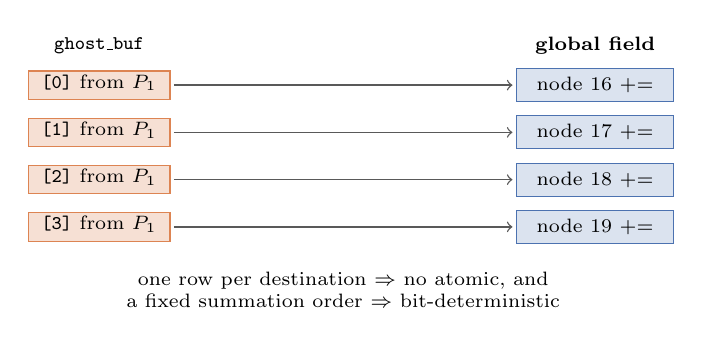
\begin{tikzpicture}[scale=1.00,font=\scriptsize]
  \node[anchor=south,font=\scriptsize\bfseries] at (1.1,2.15) {\texttt{ghost\_buf}};
  \node[anchor=south,font=\scriptsize\bfseries] at (7.4,2.15) {global field};
  \draw[PackB,fill=PackB!25] (0.2,1.70) rectangle (2.0,2.06);
  \node at (1.1,1.91) {\texttt{[0]} from $P_1$};
  \draw[PackB,fill=PackB!25] (0.2,1.10) rectangle (2.0,1.46);
  \node at (1.1,1.31) {\texttt{[1]} from $P_1$};
  \draw[PackB,fill=PackB!25] (0.2,0.50) rectangle (2.0,0.86);
  \node at (1.1,0.71) {\texttt{[2]} from $P_1$};
  \draw[PackB,fill=PackB!25] (0.2,-0.10) rectangle (2.0,0.26);
  \node at (1.1,0.11) {\texttt{[3]} from $P_1$};
  \draw[PackA,fill=PackA!20] (6.4,1.67) rectangle (8.4,2.09);
  \node at (7.4,1.88) {node $16$ $\mathrel{+}=$};
  \draw[->,black!65,line width=0.5pt] (2.05,1.88) -- (6.35,1.88);
  \draw[PackA,fill=PackA!20] (6.4,1.07) rectangle (8.4,1.49);
  \node at (7.4,1.28) {node $17$ $\mathrel{+}=$};
  \draw[->,black!65,line width=0.5pt] (2.05,1.28) -- (6.35,1.28);
  \draw[PackA,fill=PackA!20] (6.4,0.47) rectangle (8.4,0.89);
  \node at (7.4,0.68) {node $18$ $\mathrel{+}=$};
  \draw[->,black!65,line width=0.5pt] (2.05,0.68) -- (6.35,0.68);
  \draw[PackA,fill=PackA!20] (6.4,-0.13) rectangle (8.4,0.29);
  \node at (7.4,0.08) {node $19$ $\mathrel{+}=$};
  \draw[->,black!65,line width=0.5pt] (2.05,0.08) -- (6.35,0.08);
  \node[anchor=north,align=center,font=\scriptsize] at (4.2,-0.37) {one row per destination $\Rightarrow$ no atomic, and\\a fixed summation order $\Rightarrow$ bit-deterministic};
\end{tikzpicture}
}
  \caption{The ghost reduction as a gather. Contributions staged by different packs against the
    same node are summed by the single row that owns that destination. There are
    $\figPackGhostEntries$ staged entries and $\figPackReduceRows$ rows in the mesh of
    Figure~\ref{fig:decomposition}.}
  \label{fig:reduction}
\end{figure}

%================================================================================================
\section{Operator application}
\label{sec:apply}

\subsection{The two-pass algorithm}

\begin{algorithm}
\caption{Packed operator application}
\label{alg:apply}
\begin{algorithmic}[1]
\ForAll{packs $p$ \textbf{in parallel}}
  \State $A \gets 0$ \Comment{pack-private accumulator, $n_{\mathrm{pack}}(p)$ rows}
  \State gather the input fields into pack-local order
  \ForAll{elements $e$ of $p$, in increasing index}
    \State evaluate the element kernel
    \State $A[\,\text{local node}\,] \mathrel{+}= \text{contribution}$
           \Comment{plain addition, no atomic}
  \EndFor
  \State \textbf{write} $A[0 \ldots n_c)$ to the global array \Comment{assignment, not
         accumulation}
  \State \textbf{store} $A[n_c \ldots n_{\mathrm{pack}})$ into the staging buffer
\EndFor
\ForAll{reduction rows $r$ \textbf{in parallel}}
  \State $\text{global}[\texttt{dest}[r]] \mathrel{+}= \sum_{j \in \text{row } r}
         \text{staged}[j]$
\EndFor
\end{algorithmic}
\end{algorithm}

Two details of Algorithm~\ref{alg:apply} are easy to read past and both are consequences of the
ownership partition. The owned rows are \emph{assigned} rather than accumulated, because no
other pack owns them --- which also means the global array never has to be zeroed, so a full
pass over the output disappears. And the staged ghost values are \emph{stored} rather than
accumulated, because the staging slot of a given pack and ghost is written by that pack alone.

The format also changes how the input is read. A flat element sweep reads each node's input once
per incident element; the packed sweep reads it once per pack node, which for a hexahedral mesh
is roughly eight times less, and contiguously for the owned majority.

\subsection{Why the result is reproducible}
\label{sec:apply:determinism}

Floating-point addition is not associative, so a reproducible result requires a fixed summation
order, not a particular one. In this format the order is fixed by three independent properties,
and it is worth separating them because they fail independently:

\begin{enumerate}
  \item \textbf{Within a pack}, one thread walks the pack's elements in increasing index order,
        and pack membership is a pure function of the element index. The order in which a node
        receives its contributions from inside the pack is therefore the same on every run and
        at every thread count.
  \item \textbf{Across packs, for owned nodes}, there is no summation to order at all: the owned
        ranges partition the node numbering, so exactly one pack contributes.
  \item \textbf{Across packs, for shared nodes}, the reduction graph fixes the order, because
        each destination is one row and the row's terms are visited in a stored sequence.
\end{enumerate}

\noindent
No atomic appears on any of these paths, and the absence is structural: it follows from the
ownership partition rather than from a choice of synchronisation primitive.

\paragraph{Scope of the claim.} The argument above is about a processor on which a pack is
processed by a single thread, which is the setting of this paper. It does not transfer
unchanged to an implementation that splits a pack across many threads and accumulates into a
shared buffer with atomic addition: the reduction graph would still be deterministic, but the
in-pack accumulation would not, and the result would not be reproducible. Making such an
implementation reproducible requires ordering the in-pack accumulation as well --- for instance
by gathering per node from a pack-local node-to-element adjacency instead of scattering per
element. We state this because the property is easy to over-claim: it is a consequence of the
whole execution, not of the format alone.

\subsection{The alternatives, and what each fixes}
\label{sec:apply:alternatives}



The packed layout is measured against two alternatives, worth distinguishing carefully because
they fail in different places.

\paragraph{Atomic.} The flat sweep addresses nodes globally and resolves every collision with an
atomic update. It imposes no structure on the mesh at all, which makes it the natural reference
implementation, and it needs the output array zeroed first because it accumulates into it. Its
weakness is not primarily the cost of the atomic instruction --- \S\ref{sec:res:scaling} shows
it scaling perfectly respectably --- but that it fixes no summation order, so the operator is
not a function of its input in the bitwise sense.

\paragraph{Colouring.} Partitioning the packs so that no two packs of a colour share a node lets
each colour write to the global arrays directly, with neither atomics nor a reduction, at the
cost of a barrier between colours. It shares the packed layout's gather and its pack-local
indexing, and differs from it only in how the result leaves the pack. That makes the pair an
unusually clean controlled comparison, and \S\ref{sec:res:scaling} uses it as one.

Colouring also fixes a summation order and is, as measured in \S\ref{sec:res:determinism},
bitwise reproducible here. We note two qualifications rather than claim it as equivalent. The
order it fixes is a property of the colouring, so reproducibility additionally requires the
colouring itself to be constructed deterministically --- a property of the construction, not of
the layout. And the cost of the barriers is paid per application and grows with the thread
count, whereas the ghost reduction's cost is proportional to the number of shared nodes, which
is a property of the mesh. Which is preferable therefore depends on how much reduction there is
to remove: for the vector-valued operators measured here, the barriers cost more than the ghost
reduction they replace, and \S\ref{sec:res:scaling} shows that gap opening with thread count.

%================================================================================================
\section{Cost model}
\label{sec:cost}

\subsection{What each representation must read}

The three representations differ less in arithmetic than in what they must move to reach it, and
the differences are structural enough to predict an ordering before any of them is run.

\paragraph{Indices.} A flat element sweep addresses its nodes globally, so it reads one
$\SI{4}{\byte}$ index per element--node incidence --- $\SI{32}{\byte}$ per hexahedron. Inside a
pack the same connectivity is expressed in pack-local indices, and because a pack may not
address more distinct nodes than its \SI{16}{\bit} index admits, those are $\SI{2}{\byte}$
wide. The
index traffic of the element sweep is therefore halved outright. This is not a compression trick
with a decode cost: the narrower index is the one the kernel indexes with.

\paragraph{Input.} As \S\ref{sec:apply} notes, the packed sweep reads a node's input once per
\emph{pack node} rather than once per element--node incidence --- eight times less for a
hexahedral mesh --- and contiguously over the owned majority, so a field held with a stride
inside an interleaved solution vector is read at the cost of a contiguous one.

\paragraph{Output.} Because the owned ranges partition the node numbering, a pack's owned rows
are \emph{written} rather than accumulated, so the global output array never has to be zeroed
and a full pass over it disappears from every application.

\subsection{Against the assembled matrix}

\begin{table}[t]
  \centering
  \caption{\fostag{} What the operator must read per degree of freedom, excluding the solution and result
    vectors, which are identical for every representation. The assembled side carries its values
    and its sparsity pattern; the matrix-free side carries the mesh. The two mesh rows are
    measured, array by array; the assembled rows follow from the sparsity pattern.}
  \label{tab:footprint}
  %% Generated by wip/paper/python/perf_figures.py -- do not edit.
%% Regenerate with: make figures

\small
\begin{tabular}{@{}lrr@{}}
\toprule
representation & B/dof & vs.\ packed mesh \\
\midrule
packed mesh & 6.6 & --- \\
standard mesh & 7.8 & $1.18\times$ \\
\midrule
assembled matrix, \texttt{f32} & 453 & $68\times$ \\
assembled matrix, \texttt{f64} & 878 & $132\times$ \\
\bottomrule
\end{tabular}

\end{table}

\paragraph{The packed mesh is smaller than the standard one, and by less than it should be.} The
16-bit index halves the connectivity, \fpStd{} to \fpConn{}~B/dof, and the ownership and ghost
arrays spend part of that back: measured at \fpPack{} elements per pack
(Table~\ref{tab:footprint}), the packed topology is \fpImpl{} against \fpStd{}~B/dof, or
\fpImplPct{}\%. Two items account for nearly all the gap to what the format costs in principle.
The permutation between packed and unpacked numbering is \fpNodeMap{}~B/dof and the apply never
reads it (\fpWorkingPct{}\% without it); and the reduction graph's two offset arrays are 64-bit
while indexing under a million entries, so narrowing them --- which their own lengths permit
with three orders of magnitude to spare --- saves \fpReduceSaving{} more and reaches
\fpFloorPct{}\%, or \fpFloorBigPct{}\% at \fpPackBig{} elements per pack where ghosts are
proportionally fewer. The table reports the implemented figure; the floor is named, not quoted.
Coordinates are byte-identical in both and excluded; with them the ratio is \fpImplPtsPct{}\%.

The sharper contrast is with assembly. A sparse matrix--vector product does little arithmetic per
byte, so its rate is set by how much it must read, and what it reads is a stencil: $4\times4$
blocks whose count grows with the connectivity. The matrix-free side reads the mesh itself, and
Table~\ref{tab:footprint} puts the gap at more than two orders of magnitude, essentially
independent of problem size.

\paragraph{The two are not the same operator, and the comparison has to say so.}
An assembled Jacobian cannot carry the Rhie--Chow pressure-gradient sensitivity: the exact
Jacobian differentiates through the nodal gradient reconstruction, so it needs the reconstructed
gradient of the \emph{direction}, and putting that into a matrix would couple pressures beyond
nearest neighbours and destroy the one-ring sparsity the matrix is built on. The matrix therefore
\emph{lags} that term, so a matrix-free action carrying it does strictly more work than the
matrix encodes and comparing the two as one operator flatters the matrix.
Table~\ref{tab:jacfair} reports both forms.

Two consequences follow. The assembled operator is bandwidth-bound at a footprint that fits no
level of cache, which is why halving the value precision is close to its only lever; and the
matrix-free operator, reading a hundredfold less, has intensity enough that the element kernel's
arithmetic is what it must hide. \S\ref{sec:res:spmv} reports whether that happens.

%================================================================================================
\section{Experimental setup}
\label{sec:setup}

\begin{table}[t]
  \centering
  \caption{The platform. One Grace die, not the dual-die Superchip.}
  \label{tab:platform}
  \small
  \begin{tabular}{@{}lrr@{}}
    \toprule
    & advertised~\cite{NvidiaGrace2023} & measured here \\
    \midrule
    Cores & 72 Neoverse~V2 & \\
    Vector & $4\times\SI{128}{\bit}$ SVE2 & \\
    L1 / L2 per core & 64+\SI{64}{\kilo\byte} / \SI{1}{\mega\byte} & \\
    L3 shared & \SI{114}{\mega\byte} & \\
    \midrule
    Memory bandwidth & $\le\SI{500}{\giga\byte\per\second}$
      & \SI{\streamTriad}{\giga\byte\per\second} \\
    FP64 rate & \SI{3.55}{\tflops} peak & \SI{\rlPeak}{\giga\flops} sustained \\
    \bottomrule
  \end{tabular}
\end{table}

Every measurement in this paper was taken on the Grace CPU die of an NVIDIA GH200 Grace Hopper
Superchip (Table~\ref{tab:platform}), at 72 OpenMP threads with threads bound to cores, unless
a thread count is the independent variable. The memory bandwidth quoted is a STREAM triad
measured on the same node rather than a vendor figure, because it is the bound the roofline of
\S\ref{sec:res:spmv} is drawn against and the two must come from the same machine.

\paragraph{How the two measured figures were obtained.} The bandwidth is a STREAM triad,
compiled with \texttt{gcc -O3 -fopenmp -mcmodel=large} over arrays of $80\times10^{6}$ doubles
--- about \SI{1.9}{\giga\byte} in three arrays, some sixteen times the shared L3, so the triad
genuinely streams. The FP64 rate is the best of five timed $N=8192$ double-precision \textsc{gemm}
calls into \textbf{OpenBLAS 0.3.28}, the threaded build the same node resolves for the solver;
at that size the operational intensity is of order $10^3$~FLOP/byte, so the kernel is
unambiguously compute-bound and the figure is a sustained rate rather than a peak. Five
repetitions agreed to \SI{0.2}{\percent}.

\paragraph{Measured against advertised.} The triad reaches \SI{\streamTriad}{\giga\byte\per\second},
or \SI{90}{\percent} of the $\le\SI{500}{\giga\byte\per\second}$ the vendor
quotes~\cite{NvidiaGrace2023}; the \textsc{gemm} rate reaches \SI{\rlPeak}{\giga\flops}, or
\SI{65}{\percent} of the \SI{3.55}{\tflops} FP64 peak of a single Grace die. Both ratios are
ordinary --- a library \textsc{gemm} at two thirds of vector peak and a triad at nine tenths of
nominal bandwidth are what these benchmarks usually deliver --- and we draw the roofline of
\S\ref{sec:res:spmv} with the \emph{measured} pair, because the kernels being placed on it were
measured on the same node under the same conditions. Using the advertised pair would move both
roofs up and make every efficiency reported here look worse than the machine actually permits.

One further detail of the bandwidth figure: it is quoted at the thread count the kernels run at,
which is not where it peaks. The triad reaches \SI{\streamPeak}{\giga\byte\per\second} at
\streamPeakThreads{} threads and falls to \SI{\streamTriad}{\giga\byte\per\second} at
\streamThreads{} --- the memory system saturates before the socket does, so the last half of the
cores add compute but no bandwidth. We use the \streamThreads{}-thread figure throughout,
because that is the bandwidth available in the configuration being measured.

\paragraph{The case.} The operators are those of a colocated control-volume finite element
discretisation of the incompressible Navier--Stokes equations on hexahedra. Four unknowns live
at each node --- three velocity components and pressure --- and fluxes are integrated over the
sub-control-surfaces of the dual mesh. The discretisation itself is not the subject of this
paper, but \emph{which} operator is being measured is, so the variants are set out explicitly.

\paragraph{Convective schemes.} Two are measured. The baseline is \textbf{first-order upwinding
with a hard donor switch}: the face value is taken from whichever side the mass flux comes from,
with no blending band. Every measured figure and table names its scheme in the first words of
its caption, so which one produced a number is never left to be inferred.

The second is a \textbf{deferred-correction higher-order flux}. The face value is reconstructed
from the donor node and its nodal velocity gradient,
$u_{\mathrm{face}} = u_{\mathrm{donor}} + \nabla u_{\mathrm{donor}}\cdot
 (x_{\mathrm{scs}} - x_{\mathrm{donor}})$,
and only the \emph{difference} from the first-order value is added to the residual. Two
consequences follow and both matter here. The correction is residual-only, so the Jacobian stays
first-order and its assembled stencil stays at one ring --- a reconstructed face value reaches
outside the element and would otherwise regrow it to two. And the correction is lagged one
Newton step, so the nodal velocity gradient it reads is an input to the application rather than
part of it, exactly as the Rhie--Chow state gradient is. \S\ref{sec:res:convho} reports the cost
of the flux on that basis, for the unlimited reconstruction and for three limiter arms.

\paragraph{The two operators, and why the Jacobian is the exact one.} We measure the residual
$\mathcal{F}(u)$ and the action of its Jacobian $\mathcal{J}(u)\,v$, which are what a
Newton--Krylov solve applies. The Jacobian action is the \emph{exact} one, and for the
Rhie--Chow term that is a stronger statement than it sounds. The coupling depends on a
reconstructed nodal pressure gradient, so differentiating it correctly requires the
reconstructed gradient \emph{of the direction} $v$, not only of the state $u$. A lagged --- or
frozen --- Jacobian treats that gradient, and the coefficient built from it, as constant in $v$
and skips its reconstruction: cheaper per matvec, and inexact. We measure the exact form
throughout, and the driver records which one ran, so a frozen variant cannot be reported as an
exact one.

\paragraph{One-pass and two-pass operators.} Here the operators differ structurally rather than
in arithmetic. A node's reconstructed gradient needs contributions from every element incident on
it, so it must be \emph{complete} before any flux may use it --- a data dependency, not a
scheduling choice, and why the reconstruction cannot fuse into the flux sweep but is a separate
pass ending in its own ghost reduction. \textbf{One pass}: the bare element kernel, and the
residual with Rhie--Chow when the state gradient $\nabla p(u)$ is \emph{hoisted}, computed once
per Newton step and reused across the Krylov solve since $u$ is fixed there. \textbf{Two
passes}: the residual with Rhie--Chow when $\nabla p$ is rebuilt inside every application, and
the exact Rhie--Chow Jacobian action, which must reconstruct the \emph{direction}'s gradient on
every matvec because the direction changes every iteration; the driver times that pass
separately at \SI{\campQgradPct}{\percent} of the exact matvec, large enough that attributing the
whole matvec to the element kernel would misplace a sixth of it. The distinction explains two
results below: why hoisting the state gradient is worth as much as it is, and why the layout's
margin is widest on the per-apply gradient configuration of \S\ref{sec:res:ladder}, which spends
more of its time in exactly the sweep the packed layout accelerates most.

\begin{table}[t]
  \centering
  \caption{Sweeps over the mesh per operator application. Amortised sweeps run once per Newton
    step and are reused across the Krylov solve --- the nodal gradient for the hoisted and
    higher-order rows, the assembly itself for the matrix. They do not appear per application,
    but they are not free.}
  \label{tab:passes}
  \small
  \begin{tabular}{@{}lccc@{}}
    \toprule
    & element & ghost & amortised \\
    operator & sweeps & reductions & sweeps \\
    \midrule
    residual, bare                 & 1 & 1 & 0 \\
    residual, $\nabla p$ hoisted   & 1 & 1 & 1 \\
    residual, $\nabla p$ per apply & 2 & 2 & 0 \\
    residual, higher-order flux    & 1 & 1 & 1 \\
    Jacobian action, lagged RC     & 1 & 1 & 0 \\
    Jacobian action, exact RC      & 2 & 2 & 0 \\
    SpMV, assembled matrix         & 0 & 0 & 1 \\
    \bottomrule
  \end{tabular}
\end{table}

Table~\ref{tab:passes} collects the counts. Two rows deserve comment. The higher-order flux is a
one-sweep operator only because its correction is lagged; the velocity gradient it reads moves
into the amortised column rather than disappearing. And the assembled matrix performs no element
sweep at all per application --- that is the whole point of assembling --- but it pays a full
assembly, the most expensive sweep in the table, once per Newton step, and then streams a matrix
two orders of magnitude larger than the mesh on every application thereafter.

\paragraph{Optional terms.} The Rhie--Chow coupling~\cite{RhieChow1983}, which colocation
requires in order to suppress the checkerboard mode, the boundary closure over boundary
sub-control-surfaces, and the transient mass term are each switchable, and are what the
completeness ladder of \S\ref{sec:res:ladder} adds one at a time.

\paragraph{Problem sizes.} Sizes run from $n=64$ to $n=192$ on a cube, \SI{1.1e6}{} to
\SI{2.9e7}{} degrees of freedom. The smaller sizes make the saturation knee visible rather than
being compared across layouts; every cross-layout statement is drawn at $n\ge128$, where the
packed residual has saturated.

\paragraph{Measurement protocol.} Every comparison was measured inside a single allocation with
the layouts interleaved, and no figure combines runs from different nodes. This is not a
formality: node-to-node variation here is 5--11\%, larger than several differences the paper
discusses, and a change already shown performance-neutral by a controlled comparison once read
5.7--6.5\% slower with its two sides on different nodes. Each recorded run also carries the
configuration that \emph{dispatched}, not the one requested, so a measurement cannot claim a
term the code path silently dropped.

%================================================================================================
\section{Results}
\label{sec:results}

\subsection{Throughput}
\label{sec:res:throughput}

\begin{figure}[t]
  \centering
  %% Generated by wip/paper/python/perf_figures.py -- do not edit.
%% Regenerate with: make figures

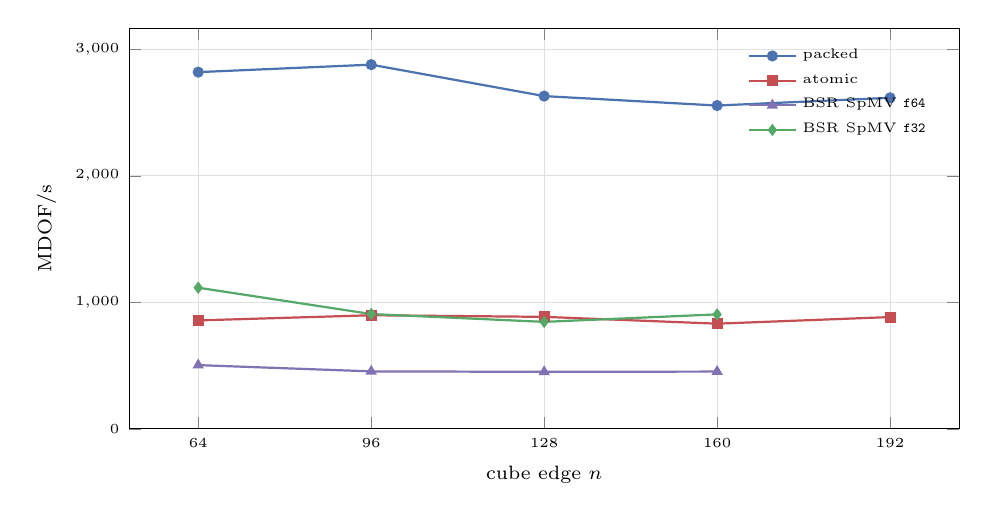
\begin{tikzpicture}
\begin{axis}[
  width=\columnwidth, height=0.55\columnwidth,
  xlabel={cube edge $n$}, ylabel={MDOF/s},
  xtick={64,96,128,160,192},
  ymin=0, legend pos=north east, legend cell align=left,
  legend style={font=\tiny, draw=none, fill=none, inner sep=1pt},
  grid=both, major grid style={black!12}, minor grid style={black!6},
  tick label style={font=\tiny}, label style={font=\scriptsize},
]
\addplot[PackA,mark=*,mark size=1.6pt,thick] coordinates {(64,2820.164) (96,2879.326) (128,2630.671) (160,2555.969) (192,2617.087)};
\addlegendentry{packed}
\addplot[PackD,mark=square*,mark size=1.6pt,thick] coordinates {(64,857.039) (96,897.824) (128,885.254) (160,831.245) (192,883.528)};
\addlegendentry{atomic}
\addplot[PackE,mark=triangle*,mark size=1.6pt,thick] coordinates {(64,503.573) (96,454.055) (128,450.439) (160,452.463)};
\addlegendentry{BSR SpMV \texttt{f64}}
\addplot[PackC,mark=diamond*,mark size=1.6pt,thick] coordinates {(64,1115.563) (96,907.441) (128,845.435) (160,904.870)};
\addlegendentry{BSR SpMV \texttt{f32}}
\end{axis}
\end{tikzpicture}

  \caption{\provwarn \fostag{} Residual throughput against problem size for the matrix-free layouts and
    for sparse matrix--vector products with the assembled matrix at both storage precisions.
    The smaller sizes show the saturation knee; cross-representation statements are drawn at
    $n\ge128$.}
  \label{fig:throughput}
\end{figure}

At the saturating size, \campDofs{} degrees of freedom, the packed residual reaches
\campResPacked{}~MDOF/s against \campResAtomic{} for the atomic sweep, and the Jacobian action
\campJacPacked{} against \campJacAtomic{}. Both are the bare element kernels here, carrying no
Rhie--Chow term; the forms that do, and the exact/lagged distinction they raise, are in
Table~\ref{tab:jacfair}. Sparse matrix--vector products with the assembled
matrix reach \campSpmvF{}~MDOF/s at double precision and \campSpmvS{} at single. Both
matrix-free layouts therefore exceed the assembled operator, and the packed one does so by a
factor of several --- which is what the footprint of Table~\ref{tab:footprint} predicts, since
the assembled product must stream two orders of magnitude more per degree of freedom.

\subsection{What the margin is, and what it is not}
\label{sec:res:ladder}

A layout comparison on a bare element kernel overstates what a solver receives. The terms a real
operator carries --- the pressure--velocity coupling, the boundary closure, the transient mass
term --- are either separate passes over the mesh or arithmetic that vectorises less well, and
both layouts pay for them, so Table~\ref{tab:ladder} reports a ladder rather than a single
ratio, adding one term at a time until the operator is the solver's.

\begin{table}[t]
  \centering
  \caption{\provwarn \fostag{} The margin as solver terms are added, residual at $n=\campN$. The bare
    element kernel is the most favourable comparison and the bottom row is the honest one.}
  \label{tab:ladder}
  %% Generated by wip/paper/python/perf_figures.py -- do not edit.
%% Regenerate with: make figures

\footnotesize
\begin{tabular}{@{}lrrrrr@{}}
\toprule
& \multicolumn{3}{c}{MDOF/s} & \multicolumn{2}{c}{packed vs.} \\
\cmidrule(lr){2-4}\cmidrule(l){5-6}
terms carried & packed & col. & standard & col. & standard \\
\midrule
element kernel & 2640 & 1863 & 1103 & $1.42\times$ & $2.39\times$ \\
${}+{}$ pressure--velocity coupling & 1787 & 1214 & 914 & $1.47\times$ & $1.96\times$ \\
${}+{}$ boundary closure & 1599 & 1087 & 864 & $1.47\times$ & $1.85\times$ \\
${}+{}$ transient term & 1457 & 1022 & 829 & $1.43\times$ & $1.76\times$ \\
\bottomrule
\end{tabular}

\end{table}

The margin falls monotonically as the operator is completed. Quoting the first row alone would
overstate what the format delivers to a solver by roughly half again.

\subsection{Reproducibility}
\label{sec:res:determinism}

\begin{table}[t]
  \centering
  \caption{\fostag{} Distinct outputs over $\detRepeats$ repeats at $72$ threads, and over one run at
    each of $\detThreads$ threads, at $n=\detN$. One distinct output means the operator is
    bitwise reproducible. The atomic sweep produces a \emph{different answer on every run}.
    Compared down a column only: packing renumbers the mesh, so fingerprints from different
    layouts are not comparable.}
  \label{tab:determinism}
  %% Generated by wip/paper/python/perf_figures.py -- do not edit.
%% Regenerate with: make figures

\begin{tabular}{llcc}
\toprule
& & \multicolumn{2}{c}{distinct outputs} \\
\cmidrule(lr){3-4}
layout & operator & repeats & thread counts \\
\midrule
\texttt{atomic} & residual & 3 / 3 & 4 / 4 \\
\texttt{atomic} & Jacobian action & 3 / 3 & 4 / 4 \\
\texttt{packed} & residual & \textbf{1} / 3 & \textbf{1} / 4 \\
\texttt{packed} & Jacobian action & \textbf{1} / 3 & \textbf{1} / 4 \\
\texttt{colored} & residual & \textbf{1} / 3 & \textbf{1} / 4 \\
\texttt{colored} & Jacobian action & \textbf{1} / 3 & \textbf{1} / 4 \\
\bottomrule
\end{tabular}

\end{table}

Table~\ref{tab:determinism} is unambiguous in both directions. The atomic sweep agrees with
itself in not one of the runs measured: three repeats at a fixed thread count gave three
different results, and four thread counts gave four. The packed layout gave a single answer
throughout, at every thread count, for both operators.

Colouring is reproducible here as well, and we report that rather than implying determinism is
what separates the packed layout from it. Both avoid atomics and both therefore fix a summation
order; what separates them is throughput (\S\ref{sec:res:throughput}), where the barrier per
colour is paid against a reduction whose volume is a vector rather than a matrix. Two caveats:
a colouring's reproducibility rests on the colouring being constructed deterministically, a
property of the construction and not the layout, and agreement over seven runs is evidence
rather than proof.

Reproducibility is measured with a fingerprint folding every output value's bit pattern, not
with a checksum. The distinction is not pedantic: a checksum is a running sum over millions of
values, so a last-bit difference on a handful of nodes falls below the total's unit in the last
place and vanishes. On this operator a checksum reported two runs identical while a per-node
comparison of the same output showed hundreds of differing doubles. Fingerprints are also
compared only \emph{within} a layout, as the caption says; operator equivalence across layouts
is a separate question, established by matching nodes on coordinates.

\subsection{Thread scaling, and where the advantage comes from}
\label{sec:res:scaling}

\begin{figure}[t]
  \centering
  %% Generated by wip/paper/python/perf_figures.py -- do not edit.
%% Regenerate with: make figures

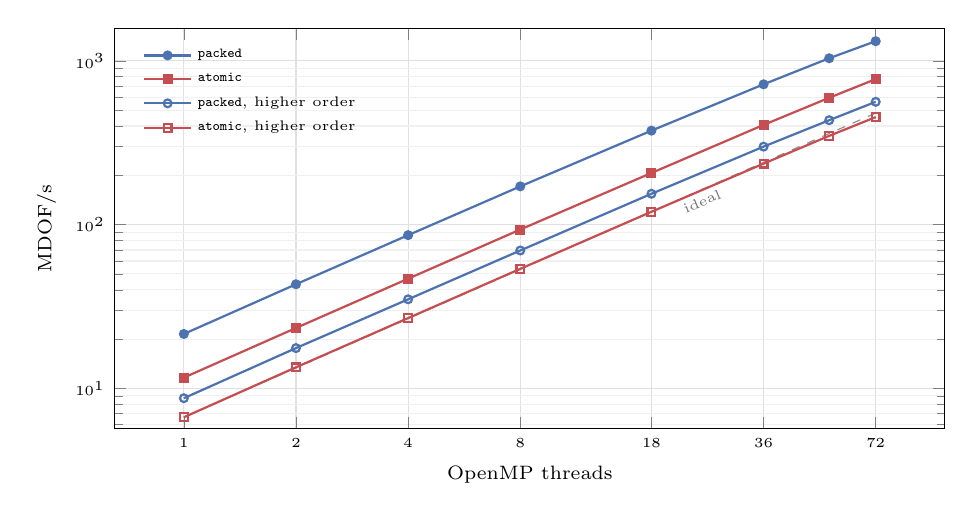
\begin{tikzpicture}
\begin{loglogaxis}[
  width=\columnwidth, height=0.550\columnwidth,
  xlabel={OpenMP threads}, ylabel={MDOF/s},
  log basis x=2, xtick={1,2,4,8,18,36,72}, xticklabels={1,2,4,8,18,36,72},
  ymin=5.6669, ymax=1581.7500,
  legend pos=north west, legend cell align=left,
  legend style={font=\tiny, draw=none, fill=none, inner sep=1pt},
  grid=both, major grid style={black!12}, minor grid style={black!6},
  tick label style={font=\tiny}, label style={font=\scriptsize},
]
\addplot[black!45,dashed,no marks,forget plot] coordinates {(1,6.6670) (72,480.0240)};
\node[black!55,font=\tiny,rotate=22.7,anchor=north,inner sep=2pt] at (axis cs:24,160.01) {ideal};
\addplot[PackA,mark=*,mark size=1.4pt,thick] coordinates {(1,21.4980) (2,43.2350) (4,86.2330) (8,171.2050) (18,374.9270) (36,718.8230) (54,1037.0530) (72,1318.1250)};
\addlegendentry{\texttt{packed}}
\addplot[PackD,mark=square*,mark size=1.4pt,thick] coordinates {(1,11.6400) (2,23.3850) (4,46.7560) (8,93.3330) (18,206.7160) (36,406.3070) (54,594.8930) (72,773.4590)};
\addlegendentry{\texttt{atomic}}
\addplot[PackA,mark=o,mark size=1.4pt,thick] coordinates {(1,8.7130) (2,17.6240) (4,35.0030) (8,69.5050) (18,154.2690) (36,299.3210) (54,434.0760) (72,562.0830)};
\addlegendentry{\texttt{packed}, higher order}
\addplot[PackD,mark=square,mark size=1.4pt,thick] coordinates {(1,6.6670) (2,13.4530) (4,26.8770) (8,53.7010) (18,119.7920) (36,235.7020) (54,348.2660) (72,453.4600)};
\addlegendentry{\texttt{atomic}, higher order}
\end{loglogaxis}
\end{tikzpicture}

  \caption{\fostag{} Residual throughput against thread count, $n=128$, \scalePacks{} packs. The packed
    and coloured curves begin at the same point and separate as barriers accumulate; the atomic
    curve begins a factor of two and a half lower and stays there.}
  \label{fig:scaling}
\end{figure}

Figure~\ref{fig:scaling} separates two effects that a single-threaded or a fully-threaded
measurement alone would confound, and the separation is worth more than the headline ratio.

\paragraph{The layout advantage is already present at one thread.} At a single thread the
packed and coloured sweeps reach \scalePackedResOne{} and \scaleColoredResOne{}~MDOF/s --- the
same number to within a per cent --- against \scaleAtomicResOne{} for the atomic sweep. That is
a factor of \num{2.5}, measured where there is no contention of any kind, and the two layouts
that share it are exactly the two that share the pack-local gather and the narrowed index
width. The advantage is therefore attributable to what the sweep \emph{reads}, as
\S\ref{sec:cost} predicts, and not to what it avoids contending on.

\paragraph{The atomic sweep does not scale badly.} It reaches
$\scaleAtomicResSpeedup\times$ on 72 threads, an efficiency of \scaleAtomicResEff\%, which is
better than the packed layout's \scalePackedResEff\%. We had expected the opposite --- that
contention on shared nodes would worsen with thread count --- and it is not what happens at this
problem size. The atomic sweep is slower throughout because each of its threads does more work,
not because its threads obstruct one another. Reporting this matters, because the common
argument for removing atomics is contention, and on this evidence contention is not what the
removal is buying.

\paragraph{What colouring costs is visible as a divergence.} The coloured sweep starts level
with the packed one and falls away steadily, ending at \scaleColoredResTop{} against
\scalePackedResTop{}~MDOF/s, an efficiency of \scaleColoredResEff\% against
\scalePackedResEff\%. Its last two points differ by only a few per cent, so it has stopped
scaling before the socket is full. This is the barrier per colour, isolated: the two layouts
differ in nothing else, so the gap between the curves is the cost of synchronising between
colours rather than reducing afterwards --- and it is the reason a ghost reduction is preferable
to a colouring when the object being reduced is a vector.

\paragraph{Why the packed curve is not ideal either.} Its efficiency of \scalePackedResEff\% has
a structural explanation rather than a mysterious one. The unit of parallel work is the pack,
and there are \scalePacks{} of them for 72 threads --- about fourteen each --- so static
scheduling quantises the imbalance in steps of roughly seven per cent before any variation in
per-pack cost is counted. That is a statement about the pack size, and \S\ref{sec:res:packsize}
takes it up.

\subsection{Pack size and the index-type ceiling}
\label{sec:res:packsize}

\begin{figure}[t]
  \centering
  %% Generated by wip/paper/python/perf_figures.py -- do not edit.
%% Regenerate with: make figures

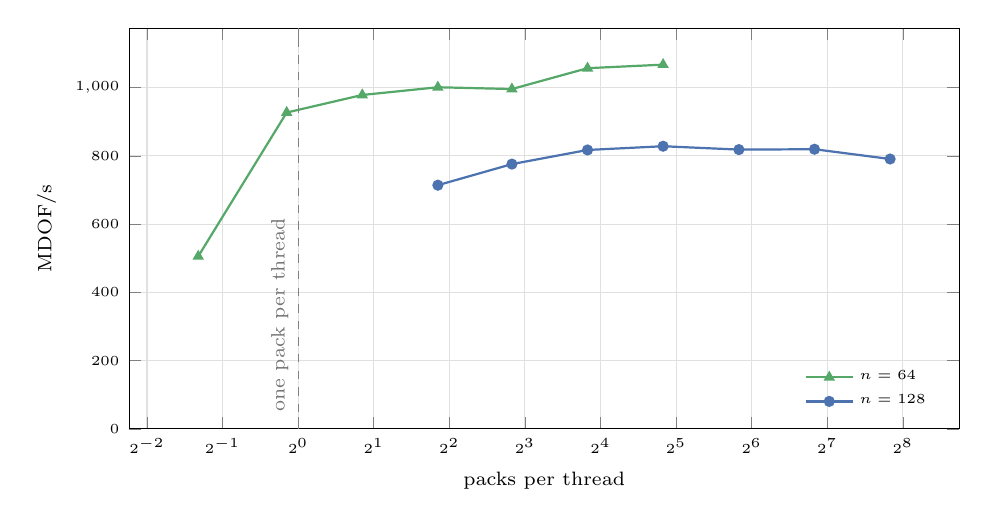
\begin{tikzpicture}
\begin{semilogxaxis}[
  width=\columnwidth, height=0.55\columnwidth,
  xlabel={packs per thread}, ylabel={MDOF/s},
  log basis x=2, ymin=0,
  legend pos=south east, legend cell align=left,
  legend style={font=\tiny, draw=none, fill=none, inner sep=1pt},
  grid=both, major grid style={black!12}, minor grid style={black!6},
  tick label style={font=\tiny}, label style={font=\scriptsize},
]
\addplot[PackC,mark=triangle*,mark size=1.6pt,thick] coordinates {(0.40,505.512) (0.90,926.846) (1.80,978.330) (3.60,1000.965) (7.10,995.709) (14.20,1056.826) (28.40,1067.205)};
\addlegendentry{$n=64$}
\addplot[PackA,mark=*,mark size=1.6pt,thick] coordinates {(3.60,713.938) (7.10,775.744) (14.20,817.140) (28.40,828.121) (56.90,818.217) (113.80,819.336) (227.60,790.656)};
\addlegendentry{$n=128$}
\draw[black!50,dashed] (axis cs:1,0) -- (axis cs:1,\pgfkeysvalueof{/pgfplots/ymax});
\node[black!55,font=\scriptsize,anchor=south west,rotate=90] at (axis cs:1,0) {\ one pack per thread};
\end{semilogxaxis}
\end{tikzpicture}

  \caption{\fostag{} Throughput of the \emph{exact} Rhie--Chow Jacobian action --- the two-sweep form,
    carrying the boundary closure --- against the number of packs per thread, at two problem
    sizes. The pack size is the knob, but packs per thread is what explains the collapse: the
    two sizes fail at the same place on this axis while failing at different pack sizes.}
  \label{fig:packsize}
\end{figure}

The pack size is the one parameter of the format, and what selects its default is not what
should. A pack may address no more distinct nodes than its index type admits, and the packer
sizes packs against that ceiling using the pessimistic bound (elements $\times$ nodes per
element), which credits no sharing at all. For hexahedra that yields roughly
$\packLargeCeil{}$ elements per pack. But a pack is one unit of parallel work, so the number of
packs \emph{is} the available parallelism, and an index-width ceiling knows nothing about how
many cores the machine has.

Figure~\ref{fig:packsize} shows what that costs. At $n=\packLargeN{}$ the ceiling-derived pack
leaves $\packLargeCeilPacks{}$ packs for 72 threads and gives up a factor of
$\packLargeCeilLoss\times$ against the best size. At $n=\packSmallN{}$ the same pack size leaves
$\packSmallCeilPacks{}$ packs --- \packSmallCeilPpt{} per thread, so most cores cannot be given
work at all --- and throughput falls by $\packSmallCeilLoss\times$. Plotted against packs per
thread the two curves fail together, which is the evidence that parallel granularity and not
cache residency is the mechanism.

The remedy is to derive the default from the core count rather than from the index width,
subject to the ceiling as a correctness bound: every configuration that performed well here had
at least fourteen packs per thread, and every configuration below one pack per thread collapsed.

\subsection{Spatial ordering is a precondition}
\label{sec:res:ordering}

\begin{table}[t]
  \centering
  \caption{\fostag{} Element order at fixed pack size, for the residual and the \emph{exact} Rhie--Chow
    Jacobian action, both carrying the boundary closure. Without a space-filling pass a pack's
    elements are scattered and its node set grows, and both operators pay for it.}
  \label{tab:ordering}
  %% Generated by wip/paper/python/perf_figures.py -- do not edit.
%% Regenerate with: make figures

\begin{tabular}{rlrrr}
\toprule
$n$ & element order & nodes/pack & residual & Jacobian \\
& & & \multicolumn{2}{c}{MDOF/s} \\
\midrule
64 & space-filling & 2601 & 1343 & 986 \\
64 & lexicographic & 4290 & 1254 & 801 \\
128 & space-filling & 2601 & 1273 & 829 \\
128 & lexicographic & 4386 & 1091 & 694 \\
\bottomrule
\end{tabular}

\end{table}

Because a pack is a contiguous range of element indices, the element order decides which nodes a
pack touches. Removing the space-filling pass at fixed pack size grows the mean node set per
pack from $\ordSfcMean{}$ to $\ordLexMean{}$ and costs $\ordSfcRes{}\to\ordLexRes{}$~MDOF/s on
the residual and $\ordSfcJac{}\to\ordLexJac{}$ on the Jacobian action
(Table~\ref{tab:ordering}). The ordering is part of the format, not an optimisation applied to
it, which is why \S\ref{sec:format} states it as a precondition.

\subsection{The higher-order convective flux}
\label{sec:res:convho}

\begin{table}[t]
  \centering
  \caption{\emph{Higher-order, deferred correction.} Cost of the flux, residual only. Each ratio
    isolates one variable: \emph{gen/hand} is two kernels at one layout, \emph{hand/atomic} one
    kernel at two layouts. The nodal velocity gradient is hoisted, so what is timed is the flux
    and not the reconstruction feeding it. Every arm's checksum differs from the first-order one,
    which is what says the correction was applied; the generator refuses the table otherwise.}
  \label{tab:convho}
  \inputifready{tables/convho}{convective scheme arms, jobs/conv\_ho\_bench.sbatch}
\end{table}

\begin{figure}[t]
  \centering
  \inputifready{figures/convho}{convective scheme arms, jobs/conv\_ho\_bench.sbatch}
  \caption{The same five variants as Table~\ref{tab:convho}. The two layouts converge from left to
    right: each added term is arithmetic per sub-control surface that the layout does not
    accelerate.}
  \label{fig:convho}
\end{figure}

The correction is not free and is not meant to be: it adds a reconstruction and, where a limiter is
selected, a limiter evaluation at every sub-control surface, against a first-order flux that is a
branch and a multiply. Table~\ref{tab:convho} and Figure~\ref{fig:convho} put all five variants on
one footing and ask the same question of each.

\paragraph{The layout's advantage falls as arithmetic per surface rises, monotonically.} It is
$\hoFirstLayoutRatio\times$ on first-order upwind, $\hoUnlimLayoutRatio\times$ once the unlimited
reconstruction is added, and $\hoDmLayoutRatio\times$ to $\hoVenkLayoutRatio\times$ with a limiter.
That ordering is the paper's own thesis read off a single table. The format accelerates what the
sweep reads and how it writes; the higher-order flux adds arithmetic per sub-control surface without
adding traffic, so with every term the share of the operator the layout can accelerate shrinks. It
is the same effect the completeness ladder measures in \S\ref{sec:res:ladder}, here driven by the
convective scheme rather than by which physical terms are switched on, and it reaches the same
conclusion: a margin quoted from the cheapest kernel is not the margin a solver receives.

\paragraph{The cost of the correction, within one layout.} Against first order in the same layout
--- so the format is not in the comparison and what remains is the scheme's own arithmetic --- the
unlimited reconstruction costs $\hoUnlimCostAtomic\times$ on atomic and the limiters
$\hoClipCostAtomic\times$ to $\hoVenkCostAtomic\times$. On packed the same corrections cost
$\hoUnlimCostPacked\times$ to $\hoVenkCostPacked\times$, more in relative terms precisely because
the layout had removed so much of the first-order cost that the arithmetic it does not touch is
what is left. The limiters separate by less than the limited--unlimited gap, sharing the
reconstruction and differing only in what is applied to the increment.

\paragraph{The higher-order flux carries the layout's properties.} The packed higher-order
sweep has the same shape as the first-order one: stage the pack's fields, accumulate into a
pack-private buffer with plain addition, write the owned rows straight out, close the ghosts
through the reduction graph. No atomic appears, and the summation order is fixed by the same
index arrays, so the reproducibility of \S\ref{sec:res:determinism} is a property of the
higher-order operator too and not something the scheme gives up.

\paragraph{Reading the table.} Each ratio isolates one variable. \emph{gen/hand} is one operator
in one layout through two kernels, so it is what generating the kernel was worth; \emph{hand/atomic}
is one kernel in two layouts, so it is what the format is worth. The first-order row carries
neither: its packed entry is the sixteen-wide first-order sweep, which is not one of the two
kernels being compared, so it is listed for scale and both of its ratios are withheld.

All three kernels are checked against one another node by node, not by checksum, and that is not
pedantry: the residual of this state sums to order \num{1e-14} and is almost all cancellation, so a
term can be present at every node and invisible in the total. They agree to \num{2e-17} on every
arm. One such check was itself defective --- it compared two sweeps where no pack had been built, so
both wrote nothing and it reported perfect agreement --- which surfaced only on deliberately
breaking a kernel and seeing it still pass.

\subsection{Against the assembled matrix}
\label{sec:res:spmv}

\begin{figure}[t]
  \centering
  %% Generated by wip/paper/python/perf_figures.py -- do not edit.
%% Regenerate with: make figures

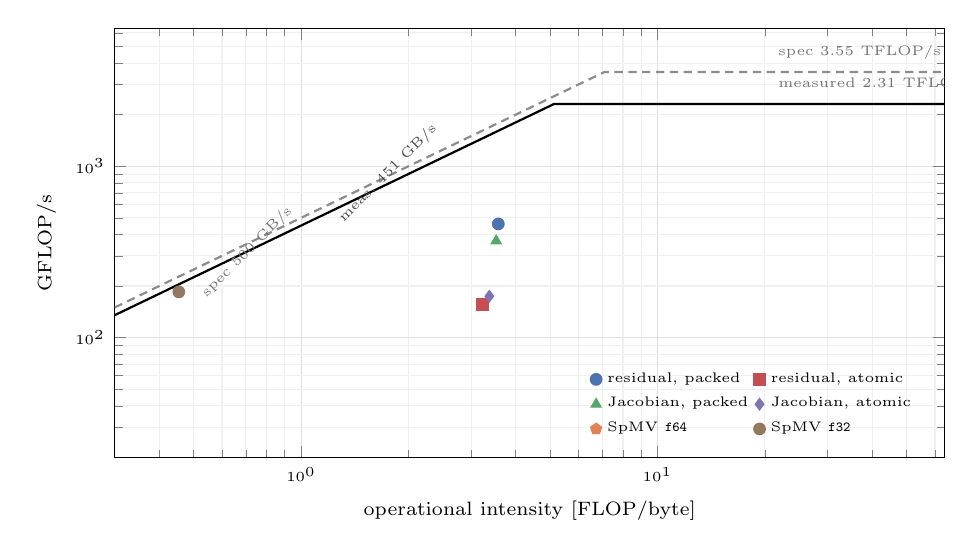
\begin{tikzpicture}
\begin{loglogaxis}[
  width=\columnwidth, height=0.58\columnwidth,
  xlabel={operational intensity [FLOP/byte]}, ylabel={GFLOP/s},
  xmin=0.3, xmax=64, ymin=20, ymax=6390,
  legend pos=south east, legend cell align=left, legend columns=2,
  legend style={font=\tiny, draw=none, fill=none, inner sep=1pt},
  grid=both, major grid style={black!12}, minor grid style={black!6},
  tick label style={font=\tiny}, label style={font=\scriptsize},
]
\addplot[black!45,thick,densely dashed,no marks,forget plot] coordinates {(0.300,150.0) (7.100,3550.0) (64.000,3550.0)};
\node[black!55,font=\tiny,anchor=south west] at (axis cs:20.48,3727.5) {spec 3.55 TFLOP/s};
\addplot[black,thick,no marks,forget plot] coordinates {(0.300,135.2) (5.116,2305.3) (64.000,2305.3)};
\node[black!55,font=\tiny,anchor=south west] at (axis cs:20.48,2420.6) {measured 2.31 TFLOP/s};
\node[black!55,font=\tiny,anchor=south east,rotate=45] at (axis cs:1.05,525.0) {spec 500 GB/s};
\node[black!70,font=\tiny,anchor=north west,rotate=45] at (axis cs:1.15,518.2) {meas.\ 451 GB/s};
\addplot[PackA,mark=*,mark size=2.1pt,only marks] coordinates {(3.575,460.8)};
\addlegendentry{residual, packed}
\addplot[PackD,mark=square*,mark size=2.1pt,only marks] coordinates {(3.223,155.7)};
\addlegendentry{residual, atomic}
\addplot[PackC,mark=triangle*,mark size=2.1pt,only marks] coordinates {(3.528,367.1)};
\addlegendentry{Jacobian, packed}
\addplot[PackE,mark=diamond*,mark size=2.1pt,only marks] coordinates {(3.374,174.5)};
\addlegendentry{Jacobian, atomic}
\addplot[PackB,mark=pentagon*,mark size=2.1pt,only marks] coordinates {(0.238,99.0)};
\addlegendentry{SpMV \texttt{f64}}
\addplot[PackF,mark=otimes*,mark size=2.1pt,only marks] coordinates {(0.454,184.9)};
\addlegendentry{SpMV \texttt{f32}}
\end{loglogaxis}
\end{tikzpicture}

  \caption{\fostag{} Both roofs measured on the same node as the points: a STREAM triad at
    \SI{\rlBw}{\giga\byte\per\second} and a large double-precision GEMM at
    \SI{\rlPeak}{\giga\flops}. The matrix-free points are the \emph{bare} element kernels, with
    no Rhie--Chow term, so the exact/lagged distinction does not arise; the SpMV points apply
    the assembled, lagged matrix. Intensity uses compulsory traffic, an upper bound, so every
    point lies at or right of its kernel's true position.}
  \label{fig:roofline}
\end{figure}

Figure~\ref{fig:roofline} places the two representations on the same axes, and the distance
between them along the horizontal is the point. The matrix-free kernels operate at
$\rlResidualPackedAi{}$--$\rlJacobianPackedAi{}$~FLOP/byte; the assembled product operates at
$\rlSpmvFSixFourAi{}$, a factor of thirty-four lower, because what it must read is a matrix
whose size grows with the stencil while the matrix-free kernels read a mesh. That is the
footprint of Table~\ref{tab:footprint} expressed as intensity, and it is why halving the value
precision --- moving the SpMV from $\rlSpmvFSixFourAi{}$ to $\rlSpmvFThreeTwoAi{}$ --- is close
to the only lever the assembled operator has.

\paragraph{The matrix-free kernel wins without being the efficient one.} It would be convenient
to report that the packed kernel is near a roof. It is not, and the assembled product is. The
ridge lies at \rlRidge{}~FLOP/byte, so the two representations are bound by different roofs, and
measured against the roof binding at its own intensity the SpMV attains \rlSpmvFSixFourPct\% ---
it is very nearly as fast as its bandwidth allows --- while the packed residual attains
\rlResidualPackedPct\% of the compute roof and the atomic sweep \rlResidualAtomicPct\%.

The packed kernel is therefore ahead not because it uses the machine better but because it plays
against a roof some twenty times higher, of which it reaches a fifth. That is the honest reading
of the figure, and it says where the remaining work is: the layout has removed the scatter as a
constraint without making the kernel either bandwidth- or arithmetic-bound, so what limits it is
neither roof but the element kernel's own instruction mix and dependencies. An assembled
operator at \rlSpmvFSixFourPct\% of its roof has almost nothing left to give; a matrix-free one
at \rlResidualPackedPct\% has a great deal.

The comparison against the atomic layout is worth reading on the same axes. Both do the same
arithmetic at the same compulsory intensity --- $\rlResidualPackedAi{}$~FLOP/byte for the
residual --- yet reach \SI{\rlResidualPacked}{\giga\flops} and
\SI{\rlResidualAtomic}{\giga\flops}. Since the model gives them identical intensity by
construction, the vertical gap is exactly what the atomic implementation adds over compulsory
traffic: re-reading each node once per incident element rather than once per pack, the global
zeroing pass, and the atomic updates themselves.

%================================================================================================
\begin{table}[t]
  \centering
  \caption{\fostag{} The Jacobian action in both forms, against sparse matrix--vector products with the
    assembled matrix. The lagged row holds the same operator the matrix does and is the
    like-for-like comparison; the exact row is what a Newton--Krylov solve should apply.}
  \label{tab:jacfair}
  \inputifready{tables/jacfair}{fair Jacobian comparison, jobs/jac\_fair.sbatch}
\end{table}

\paragraph{Against the operator the matrix can hold.} Table~\ref{tab:jacfair} separates two questions
the figure runs together. Against the operator the matrix encodes, the packed matrix-free action is
$\jfLaggedVsF\times$ the double-precision SpMV and $\jfLaggedVsS\times$ the single-precision one;
the atomic sweep is $\jfLaggedAtomicVsF\times$, barely ahead of the matrix at all. So the assembled
matrix is not far behind a \emph{poorly laid out} matrix-free operator, and the case for matrix-free
rests on the layout rather than the method alone.

Carrying the exact term costs $\jfExactCost\times$ on the packed layout, the direction-gradient
sweep appearing as throughput. Quoting the exact action against the SpMV would report
$\jfExactVsF\times$ rather than $\jfLaggedVsF\times$, understating the matrix-free side by a quarter
while appearing to favour it; both are given because they answer different questions.

\section{Discussion and limitations}
\label{sec:discussion}

\paragraph{Spatial ordering is required, not merely helpful.} Packs are contiguous element
ranges, so an unordered mesh produces packs whose nodes are scattered and numerous and the
locality the format depends on disappears. It is a precondition on the input, with a setup cost
a single application does not repay, and it renumbers the nodes in place --- which constrains
construction order downstream and makes verification against a reference match on coordinates
rather than indices. For an implicit solver applying its operator thousands of times per mesh
this is a good trade; for one evaluation it is not.

\paragraph{The determinism claim is narrower than it may appear}: \S\ref{sec:apply:determinism} scopes
it to execution in which one thread owns a pack, not to the format alone. And colouring is
atomics-free and reproducible too --- the contribution is not that the packed layout alone fixes a
summation order, but that it fixes one while also removing the barriers, both following from the
ownership partition rather than a separate mechanism.

\paragraph{The margin is a function of the operator, not a property of the format.}
\S\ref{sec:res:convho} shows it falling from $\hoFirstLayoutRatio\times$ to
$\hoVenkLayoutRatio\times$ across convective schemes, and \S\ref{sec:res:ladder} shows the same
across physical terms. A single headline ratio is only ever a statement about one operator.

\paragraph{The default pack size is chosen by the wrong constraint.} As \S\ref{sec:res:packsize}
shows, the pack size the index type admits and the one that performs best are not the same
number, and nothing in the construction reconciles them: a default set by an index-width ceiling
rather than the core count mis-sizes itself on a wide socket.

\paragraph{One node, one architecture.} Every measurement here is from a single Grace die. The
mechanisms argued for --- narrower index traffic, a gather in place of repeated indexed reads,
no zeroing pass, no atomics --- are not specific to it, but that is an argument, not a
measurement.

%================================================================================================
\section{Conclusion}
\label{sec:conclusion}

The scatter in a matrix-free operator is usually treated as a synchronisation problem. Treating
it as a data-layout problem instead --- giving every node exactly one owning pack, so that the
owned ranges partition the numbering, and closing the remainder with a gather built by sorting
--- removes the synchronisation entirely rather than making it cheaper. The operator then has no
atomic on any path and a summation order fixed by stored index arrays, so it returns the same
bits at every thread count.

Measured on the residual and Jacobian action of a colocated CVFEM Navier--Stokes discretisation on
one Grace socket, the format is faster than a standard atomic sweep and than sparse matrix--vector
products with the assembled matrix, while reading two orders of magnitude less. The thread sweep
locates the advantage: most of it is present at a single thread, where no contention exists, so it
comes from what the layout reads rather than what it avoids contending on. The margin depends on the
operator: across convective schemes it runs from $\hoFirstLayoutRatio\times$ down to
$\hoVenkLayoutRatio\times$ as arithmetic per sub-control surface grows, so a format is worth
reporting against the operator a solver applies rather than the cheapest kernel available.

\begin{acks}
The author thanks the Swiss National Science Foundation (project no.~215627), the PASC Program
(``XSES-FSI'') and USI's Fondo Istituzionale per la Ricerca; computations on Alps at CSCS.
\end{acks}

\bibliographystyle{ACM-Reference-Format}
\bibliography{refs}

\end{document}
